% MDS stuff
\label{chap-mds}
\section{Introduction}

Following the work of the previous chapter, the objective is now to find a mapping of the data into a new space which causes minimum distortion to the points in that new space. At the same time the mapping must also effectively separate those parts of the original domain which are subject to leakage. This balance (between making sure the model overcomes leakage whilst at the same time does not cause artefacts in the smooth) is essential to the success of the approach. The \sch\ transform approach, of dictating the transformed domain from the outset is clearly not flexible enough for general use. A method that depends on the shape of original domain may have more promise.

\subsection{Proposition}

Multidimensional scaling (MDS) or, as it is often referred to, principle coordinates (PCO) (\cite{gower1966}) is a method commonly used in multivariate analysis. It is closely related to techniques such as PCA (\cite{chatfieldcollins}, p. 200) and canonical correspondence analysis (\cite{terbraak}). The starting point for MDS is a matrix of distances, representing some kind of dissimilarity between observations. This distance could be calculated from the data, for example ideological distance between politicians measured using NOMINATE scores (\cite{quantss}, p. 225), or could instead be distances that occur in the data naturally through experimental setup,  for example comparative distances between stimuli response in a psychophysical experiment (\cite{torgerson}). The focus here is obviously on geographical distances.

MDS takes this matrix of distances and projects the data in such a way that Euclidean inter-point distances in the projection are approximately the same as the distances in the matrix (\cite{chatfieldcollins}, p. 187). If the matrix of distances is of rank $n$ then the projection can be in $n-1$ or less dimensions; a projection into 2 dimensions is a typical choice, since it is easily visualised. For this reason one can also think of MDS as a dimension reduction technique, finding a projection of a data cloud into lower dimensional space, while still retaining information about the dissimilarities between the points.

When MDS is performed on some categorised set of dissimilarities (as is often the case in social science and psychology) it is referred to as non-metric MDS, where as on a continuous scale it is known as metric MDS. Discussion here will focus on metric MDS.

Multidimensional scaling provides a way to transform a domain in a similar way to \sch. Given the set of distances between points in a domain, we can project those points into a configuration such that the distances between those points are approximately preserved. Now, if the Euclidean metric were to be used to calculate the distances between the points then the result from the projection would be identical (up to rotation and translation) to the starting point configuration (provided that we projected back into the same number of dimensions). However, if it were possible to use a metric that took into account the distance within the boundary (a within-area distance) then the Euclidean distances between points in the resulting configuration would be (approximately) the same as the within-area distances. This would lead to distances used by the basis functions of the smoother to be approximately the within-area distances.

Justification for this approach is as follows. In many applications within-area distances is meaningful, given that there is some reasoning behind why certain parts of the domain should not affect one another. Biological populations respect the intrinsic structure of these domains and in general do not respect Euclidean geometry in their movement patterns (for example, they move around obstacles, avoid predators and track prey). When within-area distances are meaningful, it makes sense to use this information about the structure of the domain rather than somewhat arbitrarily choose Euclidean geometry and discard this extra informaton. However, as literature on smoothing is firmly based in a Euclidean context, it would be preferable to perform the smoothing in Euclidean space. In this case the approximation to Euclidean space afforded by an MDS projection of the within-area distances offers a bridge between these two requirements.

\subsection{Proposed procedure}
\label{mdsproc}
First take the sample locations $\mathbf{x}_i = (x_{1i}, x_{2i})$ (as in \secref{intro-basic-setup}) (which for MDS could be $k$-vector, although here 2-vectors are assumed throughout this chapter) of the $i^\text{th}$ point with response $z_i$. Here, finding an MDS configuration of a set of points consists of: $i$) calculating the within-area distances between the points, $ii$) forming the distance matrix and, $iii$) actually performing the MDS projection.

The whole proposed procedure is as follows:

\begin{enumerate}
\item Obtain the MDS configuration for the domain using some representative set of points over the area in question. The only use of the MDS locations obtained in this step is to find the initial MDS configuration; they are discarded afterward. Representative points could be a sparse grid over the domain or a subset of $\{\mathbf{x}_i : i=1\dots n\}$. More detail and justification is provided in \secref{grids}, below.

\item Using the MDS configuration obtained above along with Gower's interpolation (see \secref{gowers}) to obtain the location of the sample in the MDS configuration: $\{\mathbf{x}_i^*, z_i : i=1\dots n\}$.

\item Smooth $\{\mathbf{x}_i^*, z_i : i=1\dots n\}$ using a penalised regression spline.

\item To predict at a location $\mathbf{x_j}$ in the original domain, use Gower's interpolation to obtain the point's location in the MDS space: $\mathbf{x}_j^*$. Predict $\hat{f}(\mathbf{x}_j)$.
\end{enumerate}

This approach is referred to as \mdsap\ (MultiDimensional Scaling with Regression Splines) throughout the chapter.

The rest of this chapter is structured as follows: in \secref{MDStechdet} a technical overview of MDS is given, along with technical details of how the MDS configuration is calculated; \secref{mdsdist} focuses on how the within-area distances are found; \secref{mdssims} shows some examples of this method on simulated data. Sections \ref{mds-faster} and \ref{mds-penadjust} show some improvements to the initial method and further simulations, \secref{mds-problems} details remaining problems. Finally, \secref{mds-conc} draws the chapter to a conclusion and lays out areas of further work for the next chapter.


\section{Technical details}
\label{MDStechdet}

The basic concept behind MDS as used here is to take the data, calculate their within-area inter-point distances and then find their locations in a new coordinate system based on those inter-point distances. Their new locations are determined by finding the eigen-decomposition of the (centred) matrix of distances between points. First a description of the MDS procedure when Euclidean distances are used is given, followed by the justification for the use of the same procedure when using within-area distances. 

\subsection{Finding the new point configuration}

First define $d_{ij}$ as the distance between the points $i$ and $j$. These are used to form a symmetric $n \cross n$ matrix, $\mathbf{D}$, with \ijth element $d^2_{ij}$. For the moment let us assume that $\mathbf{D}$ is known and $d_{ij}$ is the Euclidean distance between points $i$ and $j$. 

\citeb{diaconis08} gives a clear definition of the algorithm (due to \cite{schoenberg35} and \cite{torgerson}) for finding the new locations of points, which is outlined below. Further detail is given in \cite{principlesofMA}, pp. 104-108 and \cite{chatfieldcollins}, pp. 189-200.

First, suppose that the $n$ unknown new locations (in $n$ dimensions) in our MDS configuration are rows of an $n \times n$ matrix, $\tilde{\mathbf{X}}^*$. Now let $\mathbb{S}=\tilde{\mathbf{X}}^{*} \tilde{\mathbf{X}}^{*\text{T}} $, so $\mathbb{S}$ is a matrix of scalar products of the point vectors, i.e. the \ijth element of $\mathbb{S}$ is:
\begin{equation}
\mathbb{S}_{ij} = \bm{x}_i\tr{\bm{x}_j},
\label{selem}
\end{equation}
$\mathbb{S}$ is an $(n\cross n)$ matrix. Note that we may only find $\tilde{\mathbf{X}}^*$ up to a translation and rotation, so it is assumed that the values in $\tilde{\mathbf{X}}^*$ have been centred about the origin.

We now wish to relate $\mathbf{D}$ to $\mathbb{S}$. First, note that that \ijth element of $\mathbf{D}$ is 
\begin{equation}
d_{ij}^2 = (\bm{x}_i-\bm{x}_j)\tr{(\bm{x}_i-\bm{x}_j)} = \bm{x}_i\tr{\bm{x}_i} + \bm{x}_j\tr{\bm{x}_j}  -2 \bm{x}_i\tr{\bm{x}_j}.
\label{dij}
\end{equation}
Using \eqn{selem}, we can re-write \eqn{dij} as
\begin{equation}
\mathbf{D}=\text{diag}\left(\mathbb{S}\right)\tr{\bm{1}} + \bm{1}\tr{\text{diag}\left(\mathbb{S}\right)} -2\mathbb{S}.
\label{dijmat}
\end{equation}
where $\bm{1}$ is an $n \cross 1$ vector of 1s and $\text{diag}\left(\mathbb{S}\right)$ is the $n \cross 1$ vector of diagonal elements of $\mathbb{S}$.

Define:
\begin{equation}
\mathbf{H} = \mathbf{I}-\frac{1}{n}\bm{1}\tr{\bm{1}},
\end{equation}
where $\mathbf{I}$ is the identity matrix, as usual, and $\bm{1}\tr{\bm{1}}$ is an $n \cross n$ matrix of 1s.

By pre- and post-multiplying any matrix by $\mathbf{H}$ the matrix is double centred (such that row and column means are 0). Pre- and post-multiplying \eqn{dijmat} by $\mathbf{H}$ yields:
\begin{equation}
\mathbf{H}\mathbf{D}\mathbf{H} = -2\mathbf{H}\mathbb{S}\mathbf{H}.
\end{equation}
The first two terms in on the right hand side of \eqn{dijmat} are zero since the rows of $\text{diag}\left(\mathbb{S}\right)\tr{\bm{1}}$ and the columns of  $\bm{1}\tr{\text{diag}\left(\mathbb{S}\right)}$ are constant. Since $\mathbb{S}$ is already centred so $\mathbf{H}\mathbb{S}\mathbf{H}=\mathbb{S}$. Rearranging, the following relation between $\mathbb{S}$ and $\mathbf{D}$ holds:
\begin{equation}
\mathbb{S} = -\frac{1}{2}\mathbf{H}\mathbf{D}\mathbf{H}.
\end{equation}

Now there is a relation between $\mathbf{D}$ and $\mathbb{S}$, we can concentrate on dealing with $\mathbb{S}$. In order to find $\tilde{\mathbf{X}}^{*}$ we must factor $\mathbb{S}$. There are many options for matrix decomposition. One option for factoring $\mathbb{S}$ is to use the Cholesky decomposition, however, with MDS we are looking to decompose the space based on the directions of largest variation, i.e. those that have the largest contribution to $\mathbb{S}_{ij}$. For that reason we use the eigen-decomposition.

Finding the eigen-decomposition of $\mathbb{S}$, we obtain $\mathbb{S}=\mathbf{U}\mathbf{\Lambda}\tr{\mathbf{U}}$. Here $\mathbf{U}$ is the $n \cross n$ matrix orthogonal columns which are the eigenvectors of $\mathbb{S}$ and $\mathbf{\Lambda}$ is the $n \cross n$ diagonal matrix of eigenvalues of $\mathbb{S}$. Then an $\tilde{\mathbf{X}}^*$ satisfying \eqn{selem} may be computed as:
\begin{equation}
\tilde{\mathbf{X}}^*=\mathbf{U}\mathbf{\Lambda}^{\frac{1}{2}}.
\end{equation}

Following these steps $\tilde{\mathbf{X}}^*$ is an $n \cross n$ matrix. The aim here is to smooth in two dimensions, and in general multidimensional scaling is performed to reduce the dimensionality of the data, so we must now reduce the dimensionality of $\tilde{\mathbf{X}}^*$. To represent the space using two dimensions the directions with the two largest eigenvalues are chosen and the others discarded. These two largest eigenvalues and their associated eigenvectors constitute the two largest sources of variation in distance (since they are the two largest contributions to $\mathbb{S}$) this gives the two dimensional representation of the data. 

Defining $\mathbf{X}^*$ to be the $n \cross 2$ dimensional matrix obtained from truncating the full new coordinate set to the first two columns in decreasing eigenvalue order, a 2-dimensional representation has been obtained. More generally, we can find the $k$-dimensional MDS representation of the space by just taking the first $k$ columns of $\tilde{\mathbf{X}}^*$.

In summary, to calculate the MDS configuration of a set of points (given their inter-point distances) we merely need to double centre the matrix of distances, perform an eigen-decomposition on the resulting matrix, and finally truncate the eigen-decomposition and find the new point set.

For finite area smoothing, $d_{ij}$ should be the shortest distance between the points $i$ and $j$ such that the path remains within the domain. Calculation of the inter-point distances is covered in \secref{mdsdist}, however it is important to first justify the use of these steps when non-Euclidean distances are used. 

One can think of the justification in the following way: given that the distances in $\mathbf{D}$ obey the triangle inequality, all of the points from such $\mathbf{D}$ is computed ($n$ of them if $\mathbf{D}$ is $n \cross n$) may be represented by MDS in $n$ dimensional Euclidean space (at worst). Hence, in the case where the $d_{ij}$ are Euclidean distances in 2 dimensions, the smallest dimensional space in which they can be represented is 2, but they may still reside in higher dimensions. So, in the case when the distances in $\mathbf{D}$ are shortest within-area distances, one can think of the points in $\mathbf{D}$ as residing in a higher number of dimensions in such a way that the distances between them are Euclidean.

Note that an additive constant can be computed and added to the non-diagonal entries of $\mathbf{D}$ to ensure that the eigenvalues of $\mathbb{S}$ are non-negative. However, this does not occur in any of the examples shown here.

\subsection{Gower's interpolation} 
\label{gowers}
Given the setup in \secref{mdsproc}, once the MDS configuration has been found further points will need to be inserted into our MDS representation. For example when further data is collected, or in order to predict over points not in the initial grid. In this case we would like to insert those new points into the configuration given by MDS. This can be performed by Gower's interpolation (\cite{gower1968}).

Say we have some point, $x_{\text{new}}$ and we wish to find its location, $x^*_{\text{new}}$ in the MDS configuration. The position of $x^*_{\text{new}}$ is at a Euclidean distance from the points in $\mathbf{X}^*$ which is approximately the same as the within-area distance between $x_{\text{new}}$ and the points in the non-transformed space, $\mathbf{X}$. 

Note that here it is assumed that a 2 dimensional projection has been used in the initial MDS configuration, Gower's interpolation remains valid for the case in which the initial MDS projection is $k$-dimensional.

\subsubsection{Gower's interpolation formula}

We may find the position in the transformed space, $x^*_{\text{new}}$ , of some new datum $x_{\text{new}}$ in the original space using:
\begin{equation}
x^*_{\text{new}} = \frac{1}{2} \mathbf{\Lambda}^{-1} \tr{(\mathbf{X}^*)} \mathbb{D}.
\label{gower}
\end{equation}
Here $\mathbf{\Lambda}$ ($2 \cross 2$) and $\tr{(\mathbf{X}^*)}$ ($2 \cross n$) are as above, $\mathbb{D}$ ($n \cross 1$) is the vector of centred within-area distances from the points in the original configuration to $x_{\text{new}}$.

% Thesis fact: this paragraph infact represents about 3 months of work :(
In \citeb{gower1968} the $i^\text{th}$ element of $\mathbb{D}$ is defined as $-(d^2_{i,\text{new}}-\text{diag}(\tilde{X}^* \tilde{X}^{*\text{T}})_{ii})$, with $d^2_{i,\text{new}}$ being the squared distance from the $i^\text{th}$ point to the new point. The centring is given by the diagonal elements of $\tilde{\mathbf{X}}^*\tilde{\mathbf{X}^{* \text{T}}}$ i.e. the squared distances from the original points to the centroid of the MDS configuration. To avoid confusion (and to emphasise that the full $\tilde{\mathbf{X}}^*$ matrix is used, rather than its truncated version), it may be easier to think of the expression for the $i^\text{th}$ element of $\bm{d}$ as:
\begin{equation}
d_{i} = -(d^2_{i,n+1}-\text{diag}(\mathbb{S})_{ii}).
\end{equation}
Since $\mathbb{S}$ is already known, this expression is more sensible to use for computation as it doesn't imply any extra matrix multiplication.

Gower's interpolation extends simply to the case when $m$ new points are inserted by making $x^*_{\text{new}}$ as $2 \cross m$ matrix and $\mathbb{D}$ an $n \cross m$ matrix.


\subsection{Practical considerations}

Gower's paper shows that performing MDS on a dataset is equivalent to performing MDS on a reduced set of points and then inserting the remaining points, when the Euclidean metric is used to calculate the distances between the points. 

Before performing any analysis we must test that the method will be reliable and that the mapping that MDS produces  is smooth (in terms of the spatial coordinates that it produces). First, the need for using a grid as a start point for the MDS configuration is shown, and then that the mapping produces smooth lines when within-area distances are used.

\subsubsection{Using grids to compute the initial MDS configuration}
\label{grids}

To perform MDS, we must first find $\mathbf{D}$. In a spatial setting one can imagine the case in which samples were not taken from one part of the domain of interest (for example, there may be no observations in a particular peninsulae) and in that case the resulting MDS configuration would differ from when there were observations in that area. The only way that the boundary will influence the model is via the MDS configuraton and in turn, the MDS configuration's only influence from the boundary is via the distances in $\mathbf{D}$. Ensuring that different analyses on the same domain of interest yield consistent results is extremely important. 

When Euclidean distances are used to calculate $\mathbf{D}$, the critera needed so that the resulting space is the same (in the sense that the eigenvalues of $\mathbf{D}$ are the same) is that there is one more point used to create the MDS configuration than there are dimensions in the space in which they reside (provided that the points are not collinear) (\cite{landmark}). However, it is not clear what a similar criteria would be for the shortest paths used here. 

A simple example of this problem is show in \fig{tshape}. Here, a regular grid has been generated inside a T-shape (top left panel). The point configuration found by using the full set of points and within-area distances is given in the top right panel. In the pathological case when either only the ``head'' or ``tail'' of the T are sampled and used to generate the MDS and the other half inserted (bottom left for head (red) inserted from tail (black), bottom right of tail (red) inserted from head (black)), one can see that those points inserted into the configuration become warped. 

% showing the the grid is necessary using the T shape
\begin{figure}
\centering
% trim order l b r t
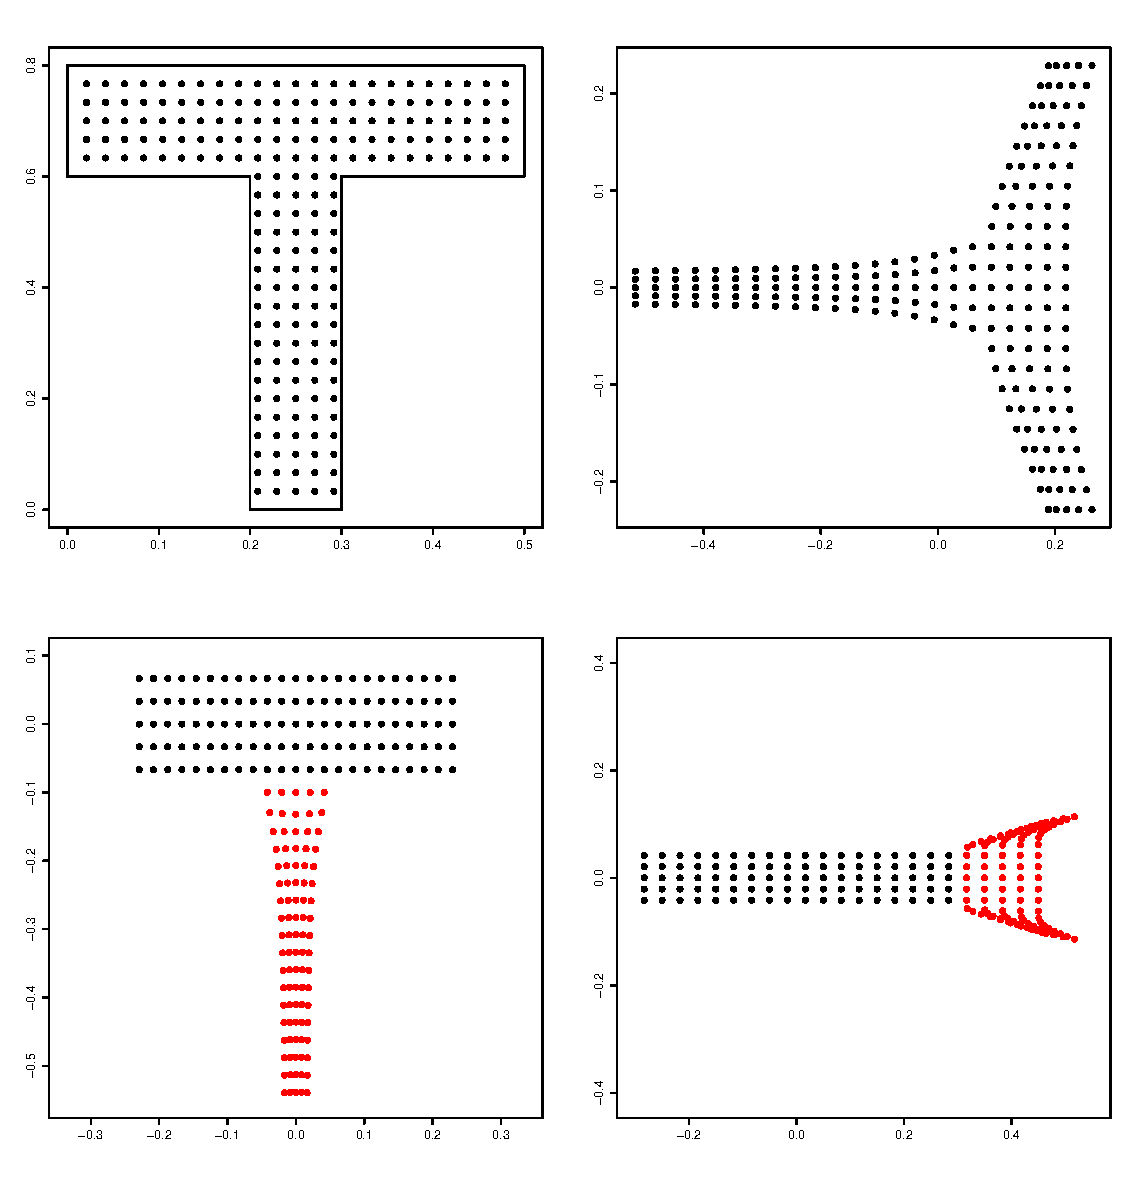
\includegraphics[width=6in]{mds/figs/tshape.pdf} \\
\caption{Data generated inside a T-shape (top left) is fed into MDS at once (top right). When either the head or tail of the T is used for the original MDS configuration and the other points inserted, the shape produced is distorted.}
\label{tshape}
% generated using figs/gridtest.R
\end{figure}

Although the cases shown in \fig{tshape} are somewhat pathological, looking at more reasonable situations still leads to wildly different results. In \fig{tshaperand} the black and green points make up the original MDS configuration; the five green points are chosen at random. The red points are then inserted. As can be seen in these four typical realisations, the shape of the MDS space is dependent on those points used to create the initial MDS configuration.

% showing the the grid is necessary using the T shape (random samples
\begin{figure}
\centering
% trim order l b r t
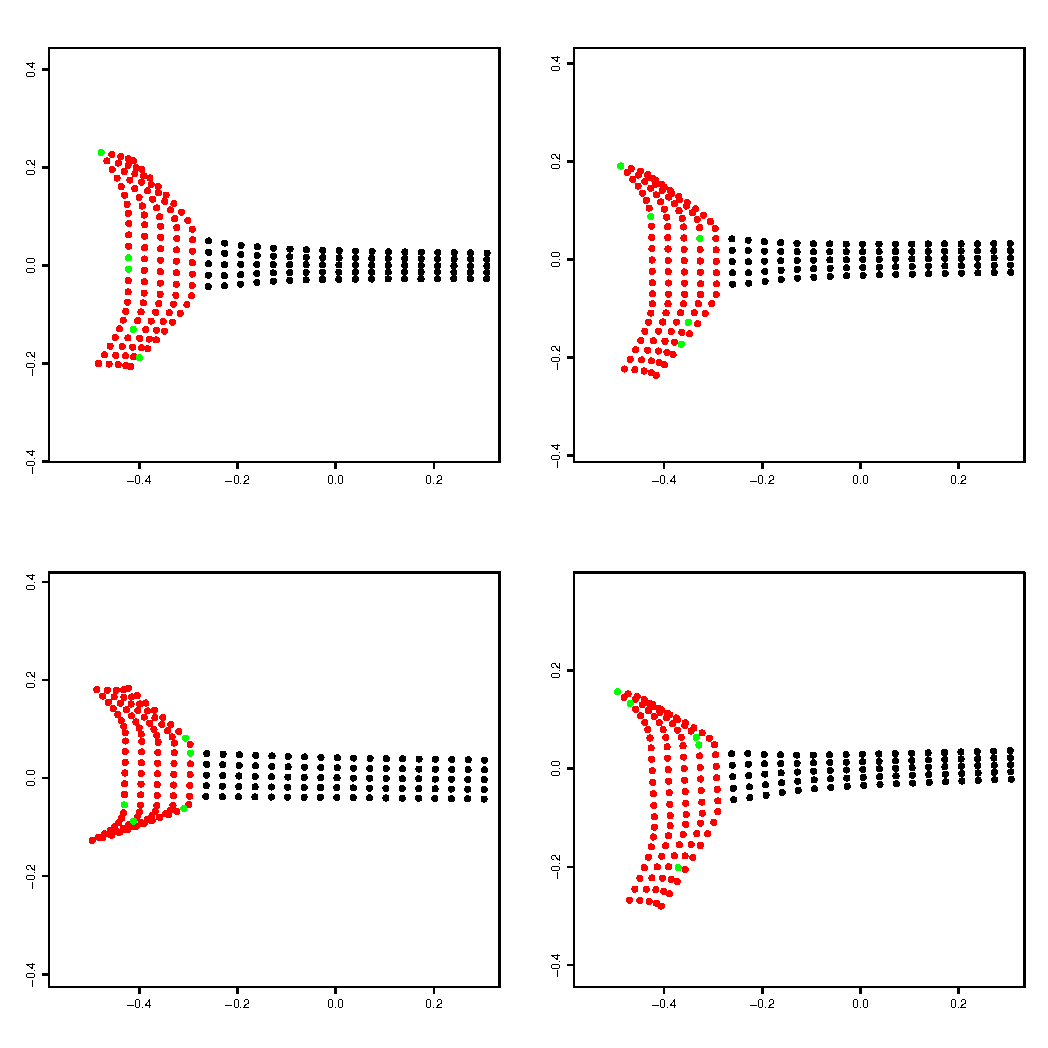
\includegraphics[width=6in]{mds/figs/tshaperand.pdf} \\
\caption{Using the T-shape in \fig{tshape} (top left), the tail (black points) of the T was used with 5 randomly sampled (green) points in the head. The head (without the 5 green points) was then inserted into the MDS configuration (red). As can be seen from these four realisations, the output varies greatly depending on the points sampled.}
\label{tshaperand}
% generated using figs/gridtest.R
\end{figure}

Hence, although there are the usual problems with predicting outside of the data, the added problem of the instability of MDS insertion can only confound results further (\cite{gower1968}).

This problem can be rectified by using an appropriately spaced grid over the domain to calculate the eigen-decomposition, thus ensuring that the whole domain is covered. The base MDS configuration is then stable, provided that the grid is fine enough to catch all of the important features in the boundary of the domain.

\subsubsection{Smoothness of mapping}
\label{mds-smoothness}

Following from this, it is important to make sure that the MDS space is smooth in the sense that a grid of smooth lines over the domain are mapped to a series of smooth lines without discontinuities or sudden changes in direction. Taking the evenly spaced 50 by 50 point grid in \fig{wt2-grid-orig}, first MDS is performed on a dense point set of size 1253, and then a less dense grid is inserted using the method of Gower. The grid produced under the insertion can be seen in \fig{wt2-grid-full}. Taking a sample of 250 points from the 1253, an MDS configuration was also found and the same grid inserted (see \fig{wt2-grid-samp}). From this it is clear that those points mapped into the domain are smooth but in the sample case the features in the far right of the shape (the less pronounced peninsulae) are slightly squashed.

% grid to map
\begin{figure}
\centering
% trim order l b r t
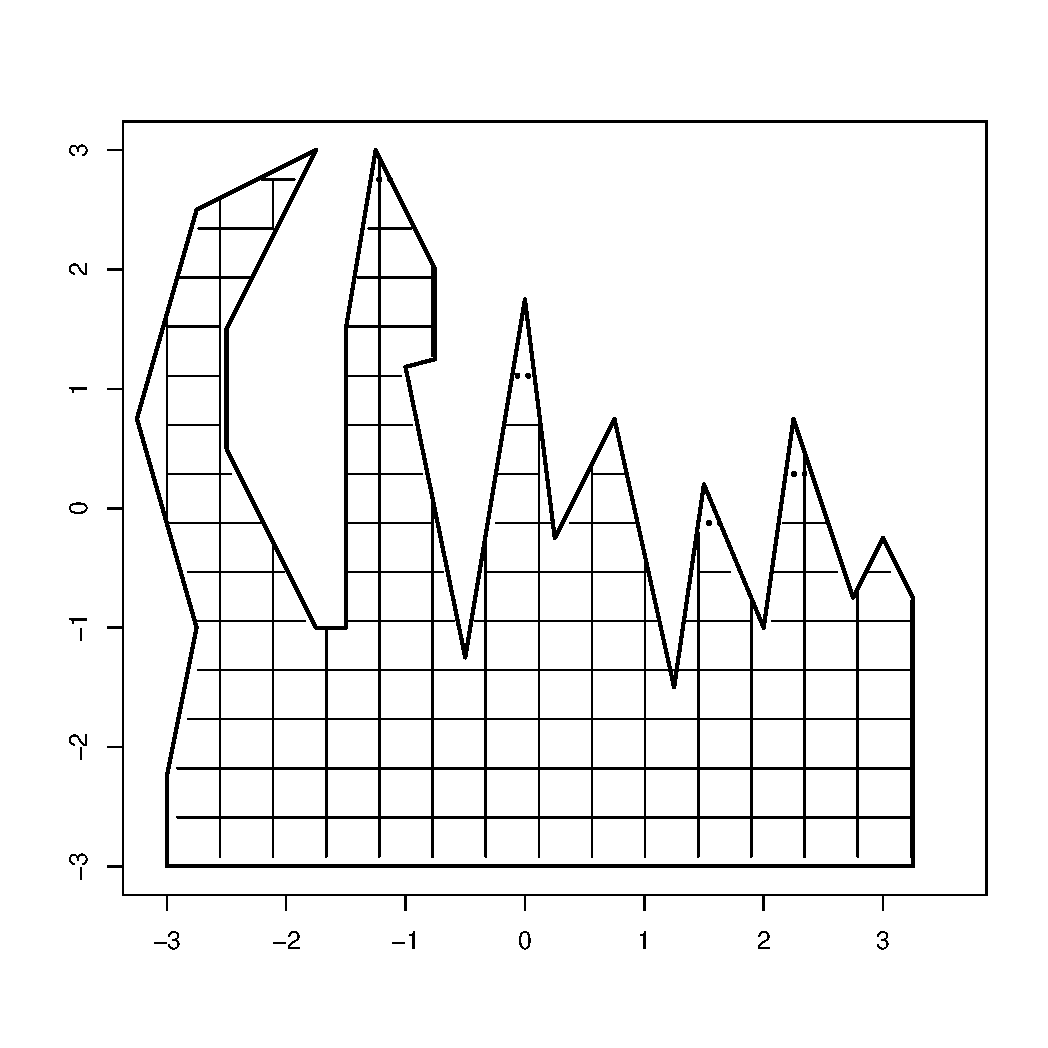
\includegraphics[width=4in]{mds/figs/wt2-grid-orig.pdf} \\
\caption{The grid to be inserted into the MDS configuration over the peninsula domain to test the smoothness of the mapping.}
\label{wt2-grid-orig}
% generated using wt2-grid.R
\end{figure}

% mapped grid (full)
\begin{figure}
\centering
% trim order l b r t
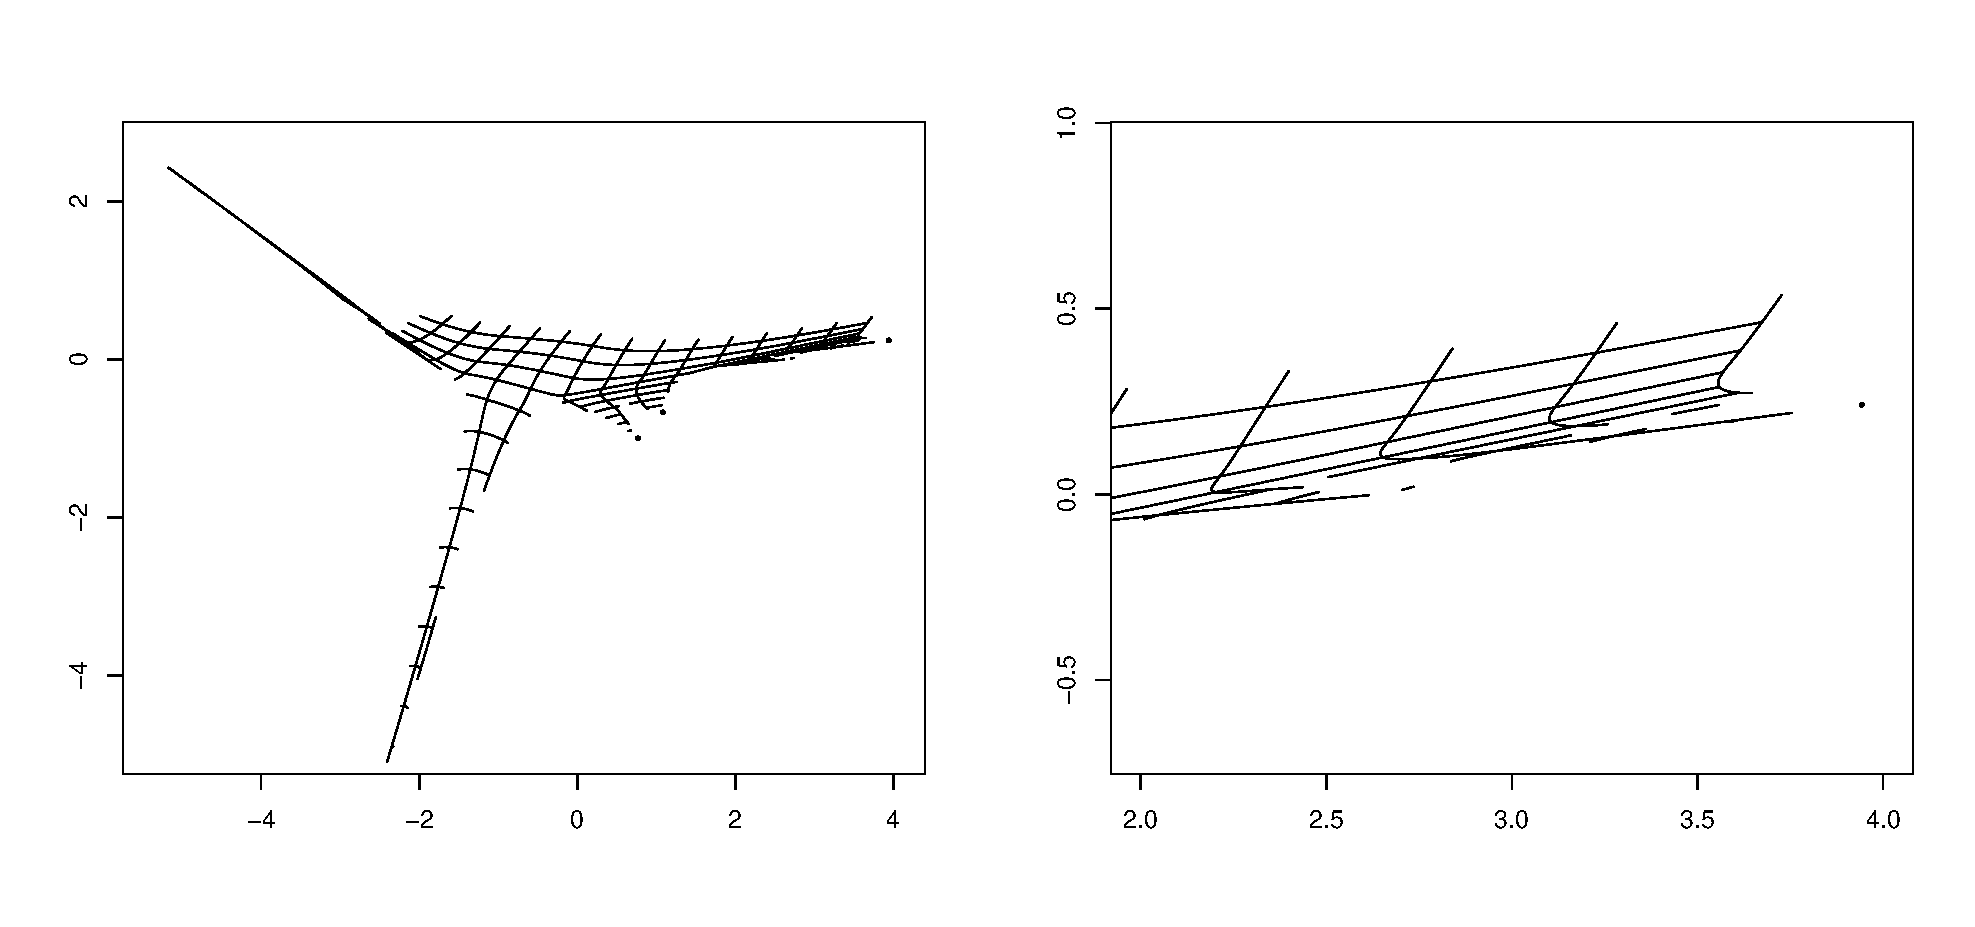
\includegraphics[width=5in]{mds/figs/wt2-grid-full.pdf} \\
\caption{Inserted grid when 1253 points are used to create the initial MDS configuration. The right panel shows a zoom of the far right part of the configuration.}
\label{wt2-grid-full}
% generated using wt2-grid.R
\end{figure}

% mapped grid (samp)
\begin{figure}
\centering
% trim order l b r t
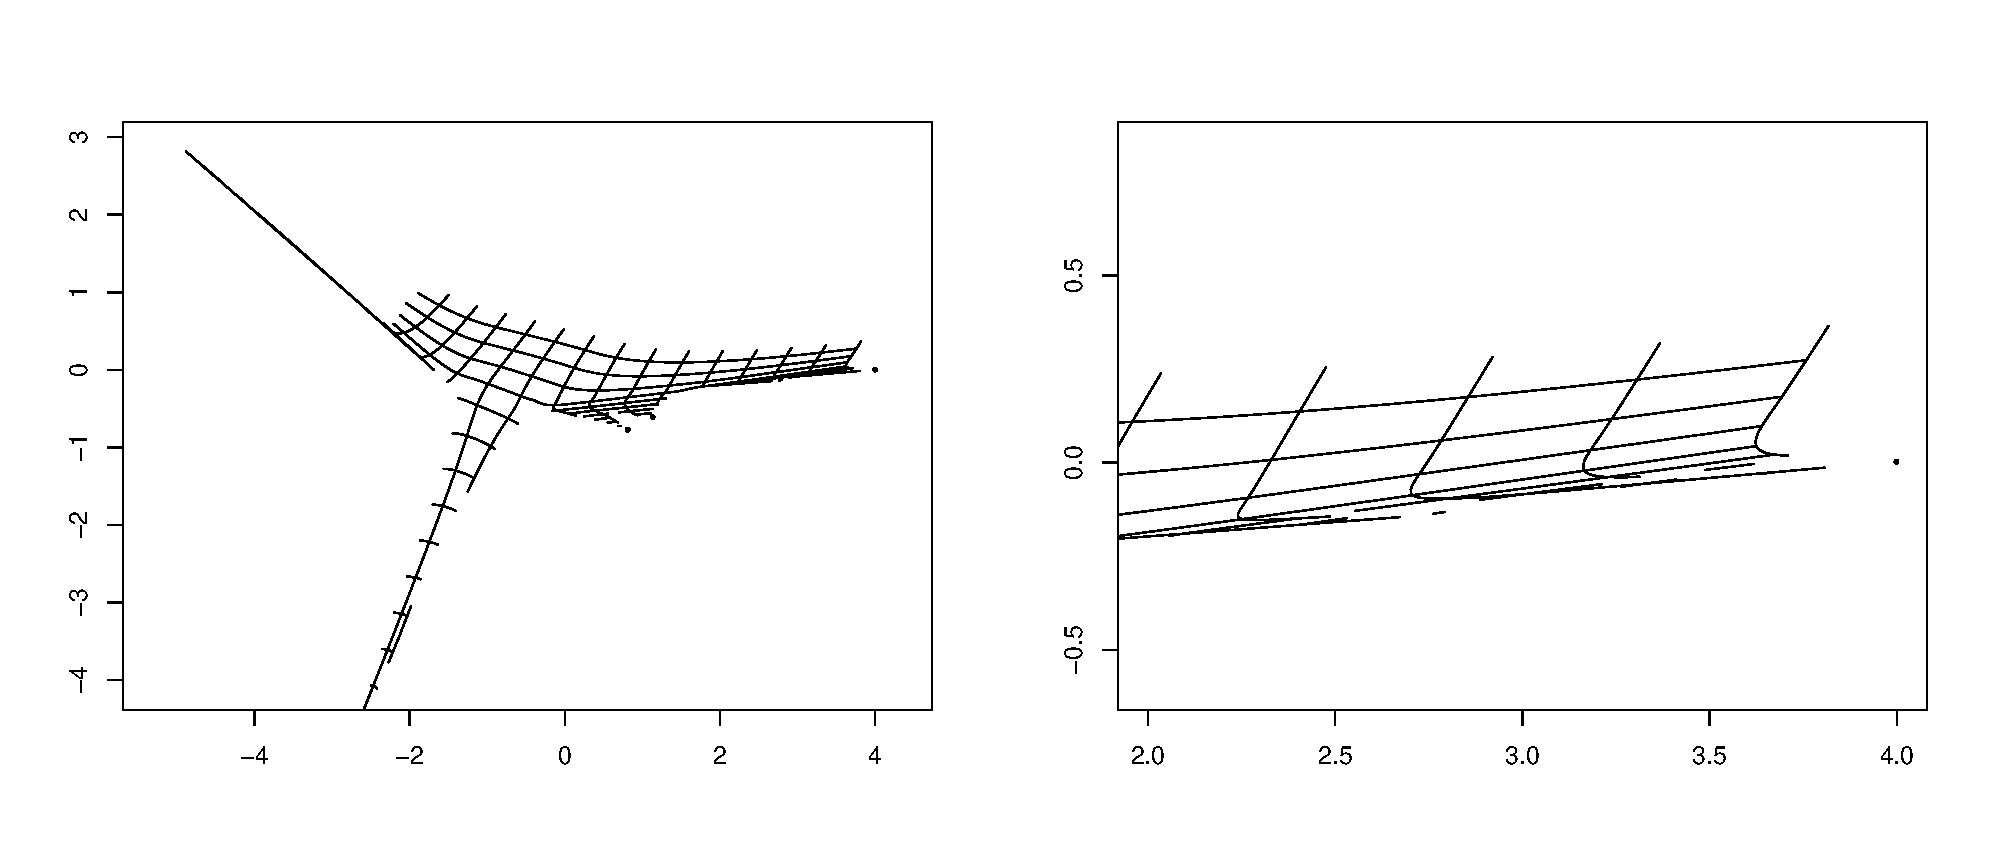
\includegraphics[width=5in]{mds/figs/wt2-grid-samp.pdf} \\
\caption{Inserted grid when 250 randomly chosen points are used to create the initial MDS configuration. The right panel shows a zoom of the far right part of the configuration. Comparing this to that of \fig{wt2-grid-full}, one can see that the features on the right have been slightly squashed together.}
\label{wt2-grid-samp}
% generated using wt2-grid.R
\end{figure}

In conclusion, the mapping can be both reliable and also produces a smooth configuration of points provided that the initial MDS configuration covers the space in sufficient detail.


\section{Finding the within-area distances}
\label{mdsdist}

So far we have assumed that the matrix of distances $D$ is known, this section describes (what the author believes to be) novel algorithm to find the within-area distances.

In order to perform MDS, the matrix of distances must be found. Euclidean distances would lead to the original configuration of points being recovered (up to translation and rotation) provided the projection dimension was the same as that of the original set of points. As was pointed out in \secref{intro-FAS}, Euclidean distances are the cause of leakage in the first place, since they do not reflect the distances that must be travelled between points residing in the domain of interest.

Note that paths between point pairs in simple polygons (i,e. those polygons without holes) are considered. Although this limits the types of domains that can be addressed, it does make the shortest path algorithm simpler, since the shortest path is unique (see appendix \ref{app-unique-sp}).

There are several methods available to calculate within-area distances, however given that the domain of interest is any arbitrary simple polygon this limits the number that are applicable. The two most promising possibilities are the geodesic methods used by \cite{wangranalli} (see also \secref{intro-leakageapproaches}) and the $\text{A}^*$ algorithm (\cite{astarpaper}) which is a generalisation of Dijkstra's algorithm (\cite{dijkstra}). However, both of these algorithms rely on the discretization of the domain of interest. As stated in \secref{intro-leakageapproaches}, this discretization of the domain is undesirable since the results then become dependent on the resolution of the discretization of the domain, even if a high enough resolution can be used the computational cost becomes prohibitively expensive for such methods. It would be preferable to have an elementary (ie. not relying on complex data structures or theory) algorithm for finding the shortest path within the polygon.

Let the domain boundary be some polygon, $\Gamma$. Given that there is no direct path within the domain between two points ($p_1$ and $p_2$, say), the algorithm proceeds as follows to create a path (ie. an ordered set of edges and vertices), $\mathcal{P}$:

\begin{enumerate}
\item (INIT) Start by drawing a line between $p_1$ and $p_2$ (\fig{wdia}, ($i$)). Start the path as the lines from $p_1$, $p_2$ to their nearest intersection with the boundary of $\Gamma$ ($p_1^1$, $p_2^1$, say). Then form two paths. The first path from $p_1^1$ to $p_2^1$ ($\mathcal{P}_1$) contains the vertices of $\Gamma$ found moving along the boundary from $p_1^1$ to $p_2^1$. The second ($\mathcal{P}_2$), is found by taking the path from $p_1^1$ to $p_2^1$ in the other direction around the boundary, ie. the vertices of $\Gamma$ not in the first path. It is easy to see that $\{\mathcal{P}_1 \cup \mathcal{P}_2\} \setminus \{p_1^1, p_2^1\} = \Gamma$. The DELETE step (below) is then performed on $\mathcal{P}_1$ and $\mathcal{P}_2$, removing any superfluous vertices. Finding the length of $\mathcal{P}_1$ and $\mathcal{P}_2$ and choosing the shorter ($\mathcal{P^*}$), the initial path is formed as $\mathcal{P}=(p_1,p_1^1,\mathcal{P}^*,p_2^1,p_2)$. 

In \fig{wdia}, ($iii$), $\mathcal{P}_1$ is marked in green and is chosen to form the initial path, $\mathcal{P}=(p_1,p_1^1,\mathcal{P}_1,p_2^1,p_2)$, as $\mathcal{P}_1$ is shorter than $\mathcal{P}_2$, in red.

\item (DELETE) Given a triple of vertices, $(v_i, v_{i+1}, v_{i+2}) \in \mathcal{P}$ , if the line between $v_i$ and $v_{i+2}$ is shorter than the path $(v_i, v_{i+1}, v_{i+2})$ and the line between $v_i$ and $v_{i+2}$ lies inside $\Gamma$ then delete $v_{i+1}$ (\fig{wdia}, ($iv$) and ($vi$)). The entire path is iterated over deleting all superfluous vertices until there are no changes in successive runs. 

For example in \fig{wdia} ($iii$), $v_2$ is deleted from $\mathcal{P}$ because the path straight between $v_1$ and $v_3$ is shorter, and within $\Gamma$.

\item (ALTER) Given a triple of vertices $(v_i, v_{i+1}, v_{i+2}) \in \mathcal{P}$, if the candidate replacement path $\mathcal{P}_{ID}$ is shorter than the path $(v_i, v_{i+1}, v_{i+2})$ then replace $(v_i, v_{i+1}, v_{i+2})$ with $\mathcal{P}_{ID}$ (\fig{wdia}, ($v$)). The candidate replacement path, $\mathcal{P}_{ID}$, is calculated by running INIT with $p_1$ and $p_2$ replaced by $v_i$ and $v_{i+2}$, producing $\mathcal{P}_I$, and then using DELETE on $\mathcal{P}_I$ to remove superfluous vertices, giving $\mathcal{P}_{ID}$.

For example in \fig{wdia} ($iv$), the path $(v_1, v_2, v_3)$ is longer than the path $\mathcal{P}_{ID}=(v_1, v^1_2, v_3)$ (green dashed line in ($iv$)) so the former is replaced with the latter in $\mathcal{P}$. The path created by INIT is marked as $\mathcal{P}_{I}$ in  ($iv$) in red.

\item (ITER) We then iterate further DELETE and ALTER steps (in pairs) until there has been no change in $\mathcal{P}$ from one run to the next (ie. convergence) (\fig{wdia}, ($vi$)).
\end{enumerate}

% diagram for finding the shortest path in W
\begin{sidewaysfigure}
\centering
% trim order l b r t
\psfrag{exp1}[]{$\mathcal{P}_1$}
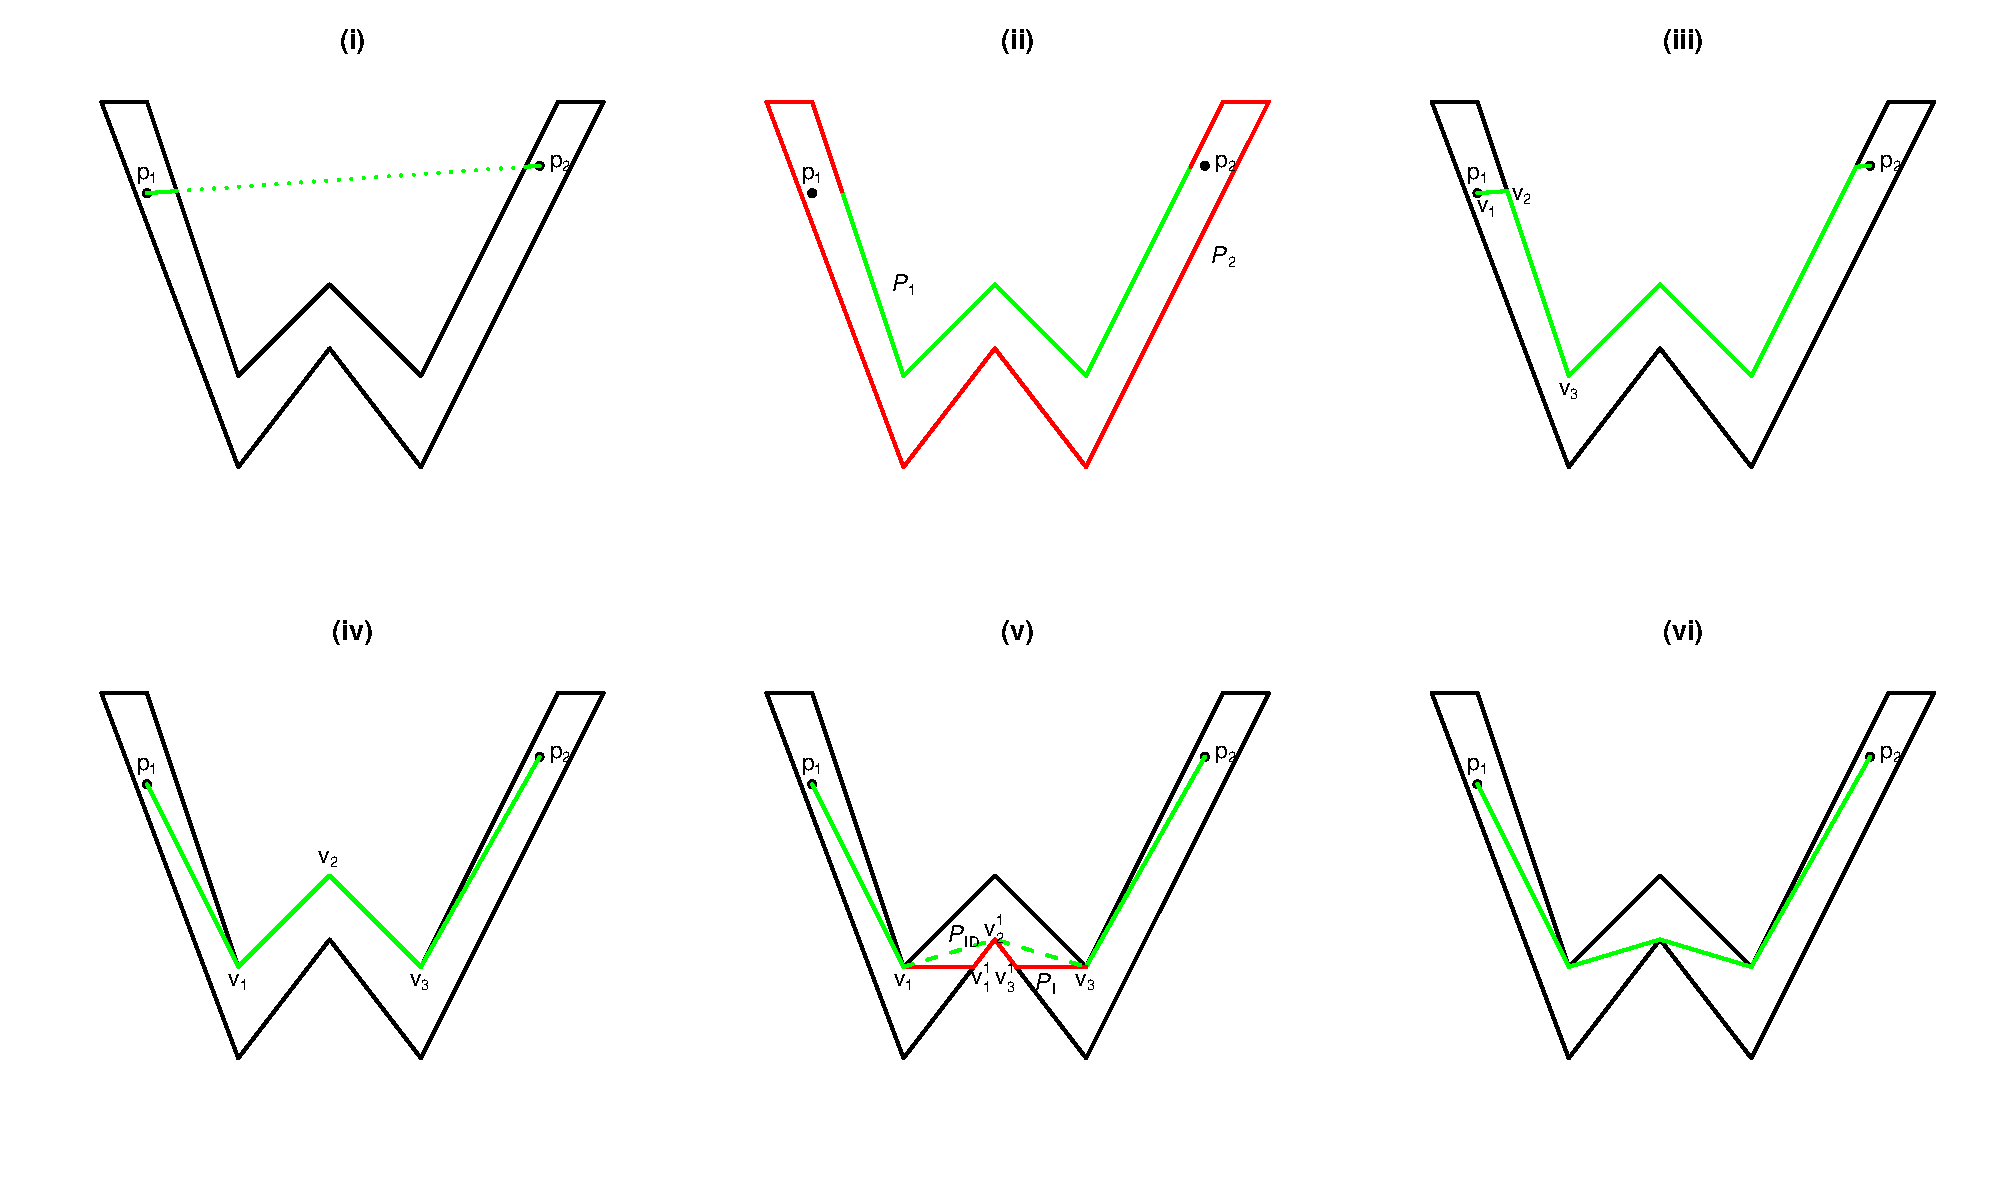
\includegraphics[trim=0in 0.5in 0in 0.25in, width=9.5in]{mds/figs/wdia.pdf} \\
\caption{The green lines in ($i$) to ($vi$) show the steps forming the shortest path as the algorithm progresses from initial state to final, shortest path (bottom right). See \secref{mdsdist}.}
\label{wdia}
% generate /phd-smoothing/mds-writeup/figs/distanceexplanation.R
\end{sidewaysfigure}

Of course, if there is a direct path between $p_1$ and $p_2$ then the Euclidean distance between the points can be used.

Further theoretical properties of this algorithm can be found in \appref{app-WAD}.

\section{Simulation experiments}
\label{mdssims}

In order to investigate the efficacy of \mdsap, a series of simulation experiments were performed. In all cases the results for \mdsap\ were compared to those of the current best method (the soap film smoother) and the standard approach that does not account for leakage (\tprs).

The \textsf{R} packages \texttt{mgcv} and \texttt{soap} with additional bespoke software for finding the within-area distances were used. In all cases smoothing parameter estimation was performed using GCV (see \secref{GAMfitting}).

\subsection{The Ramsay horseshoe}

If a general method is to be useful it must first perform well on even a simple case such as the modified Ramsay horseshoe since it clearly illustrates the problem of leakage.

\subsubsection{Setup}

For the horseshoe, samples of 250 points with normal errors (at 3 levels: 0.1, 1 and 10) were taken. (These are the settings used in \cite{soap}.) Using these samples, three models were fitted to the data. Predictions were then made over 718 points (including the sample locations). 200 realisations were generated and the EDF and MSE recorded for each replicate. The three models fitted were as follows:

\begin{enumerate}
\item \emph{Thin plate spline}: bivariate \tprs\  with basis size 100.
\item \emph{Soap film smoother}: 32 knots evenly spread over a grid over the domain, cyclic spline on the boundary was of basis size 39.
\item \emph{\mdsap}: Used a thin plate spline of basis dimension 100. The initial MDS grid was 20 points wide by 10 points tall.
\end{enumerate} 

Note that due to time and computational restrictions, the boundary was reduced from the 160 vertex polygon in the \texttt{fs.boundary()} function in \texttt{soap} to a 21 vertex polygon by only using every 8$^\text{th}$ vertex. This should not cause a major difference in results even if the soap film used the full boundary and \mdsap\ used only the reduced set of edges, since objective is to allow the smoother to get a broad idea of the topology of the domain, rather than the minutiae of the boundary features. In the simulations presented here, the soap film smoother and \mdsap\ used the same boundary.

\subsubsection{Results}

Predictions from a typical realisation can be seen from \fig{mds-ramsay-fit-1}, where the noise level was 1 with a sample size of 250. Both the soap film smoother and \mdsap\ are able to reproduce the main features of the true horseshoe function due to their ability to respect the boundary (in the case of the soap film) or the geometry of the domain (in the case of \mdsap). The \tprs\ shows leakage as expected. When the noise level is high the \mdsap\ outperforms the soap film smoother in MSE terms (and is less variable).

%\begin{table}[t]
%\centering
%\begin{tabular}{c c c c}
% & & MSE & \\ 
%Noise level & \mdsap & Soap film & Thin plate\\ 
%\hline
%0.1  & 0.0032 (3$\cross10^{-5}$) & 0.0022 (3$\cross10^{-5}$) & 0.0402 (0.0008) \\ 
%1  & 0.0436 (0.0015) & 0.0482 (0.0014) & 0.2306 (0.0024) \\ 
%10  & 2.065 (0.121) & 3.070 (0.238) & 3.371 (0.113) \\ 
%\end{tabular}
%\begin{tabular}{c  c c c }
%&  & EDF & \\ 
%Noise level & \mdsap & Soap film & Thin plate\\ 
%\hline
%0.1 & 47.613 (0.35) & 39.164 (0.26) & 92.6 (0.102)\\ 
%1  & 8.383 (0.345) & 11.868 (0.401) & 46.607 (0.424)\\ 
%10 & 5.058 (0.332) & 5.586 (0.288) & 5.979 (0.251)\\ 
%\end{tabular}
%\caption{Mean MSE and estimated degrees of freedom (EDF) for the three models fitted to the modified Ramsay horseshoe function with standard errors (in brackets) over 200 realisations. Sample size was 250 with noise levels given above.}
%\label{ramsayresultstable}
%\end{table}

The EDFs in figure \ref{edf-mds-ramsay-boxplot} show that \mdsap\ fits a less complex model than the thin plate spline on average, and for the two higher error situations, has a lower EDF than the soap film. Given that this is coupled with a lower MSE, it appears that \mdsap\ simultaneously yields both a more accurate and less complex model than the soap film for the horseshoe when there is a high level of noise. When noise is lower, the soap film and \mdsap\ MSEs are still roughly of the same order. \Fig{mds-ramsay-boxplot} shows the logarithm of the per-realisation average MSE for each of the models at each error level.

% boxplot for Ramsay
\begin{figure}
\centering
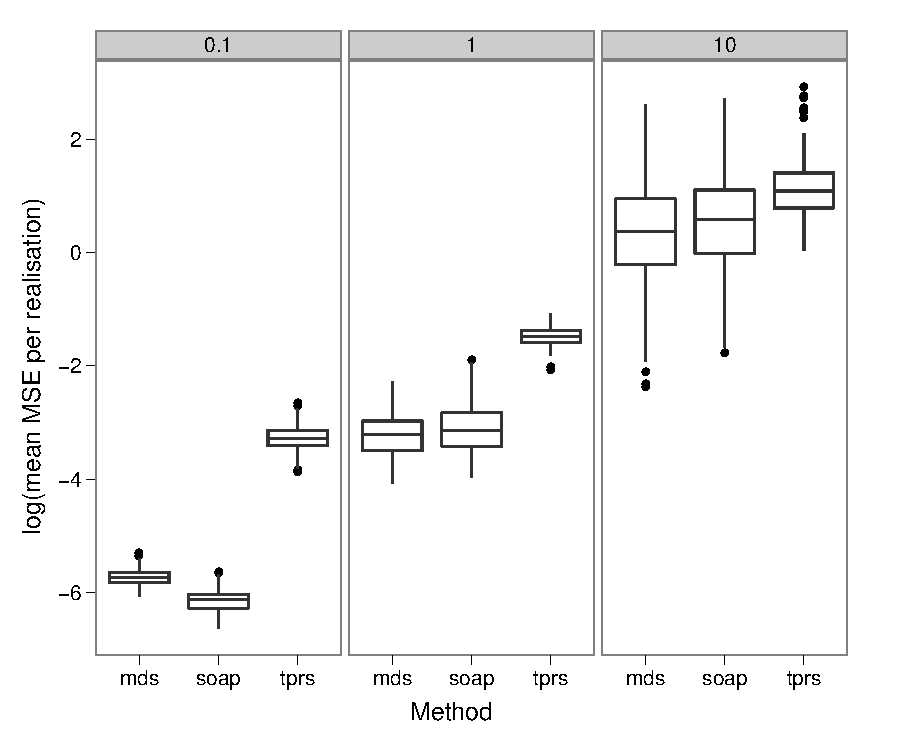
\includegraphics[width=6in]{mds/figs/mds-ramsay-boxplot.pdf} \\
\caption{Boxplots of the logarithm of the MSE per realisation of the Ramsay horseshoe for \mdsap\ (``mds''), the soap film smoother (``soap'') and \tprs\ (``tprs'') for noise levels 0.1, 1 and 10 (left to right). As previously a paired Wilcoxon signed rank test showed that MSEs for \mdsap\ and \tprs\ were significantly different from the soap film smoother (at the 0.01 level) where the colours above indicate whether the MSE was better (green) or worse (red).}
\label{mds-ramsay-boxplot}
% generated using phd-smoothing/mds/sim/boxplot-ramsay.R
\end{figure}

\begin{figure}
\centering
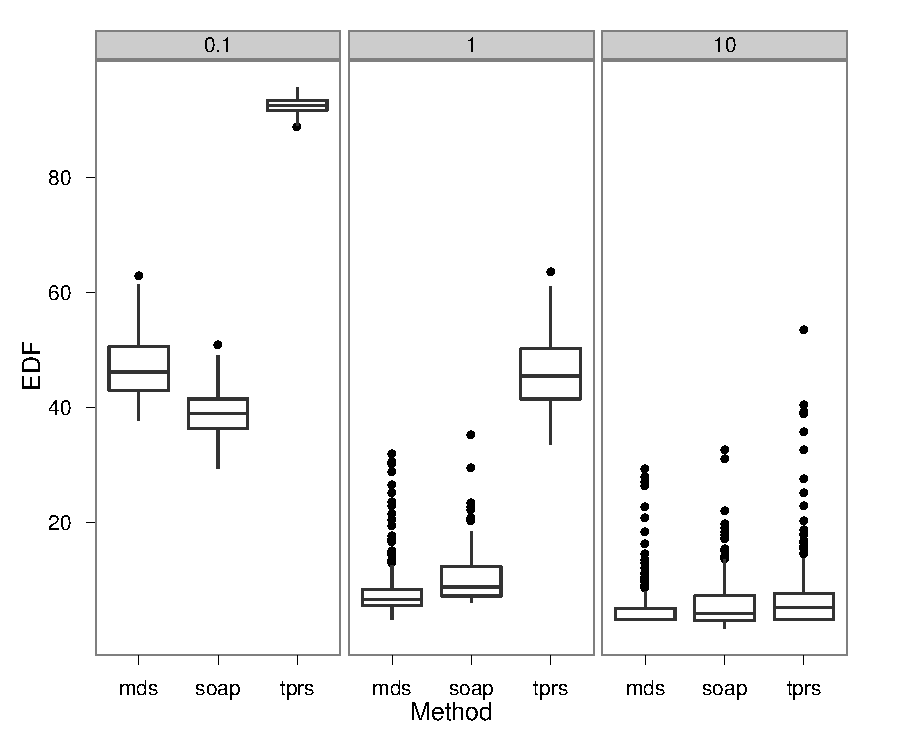
\includegraphics[width=6in]{mds/figs/edf-mds-ramsay-boxplot.pdf} \\
\caption{Boxplots of the EDF per realisation of the Ramsay horseshoe for \mdsap\ (``mds''), the soap film smoother (``soap'') and \tprs\ (``tprs'') for noise levels 0.1, 1 and 10.}
\label{edf-mds-ramsay-boxplot}
% generated using phd-smoothing/mds/sim/boxplot-ramsay-edf.R
\end{figure}


% Ramsay fit with error=1 
\begin{figure}
\centering
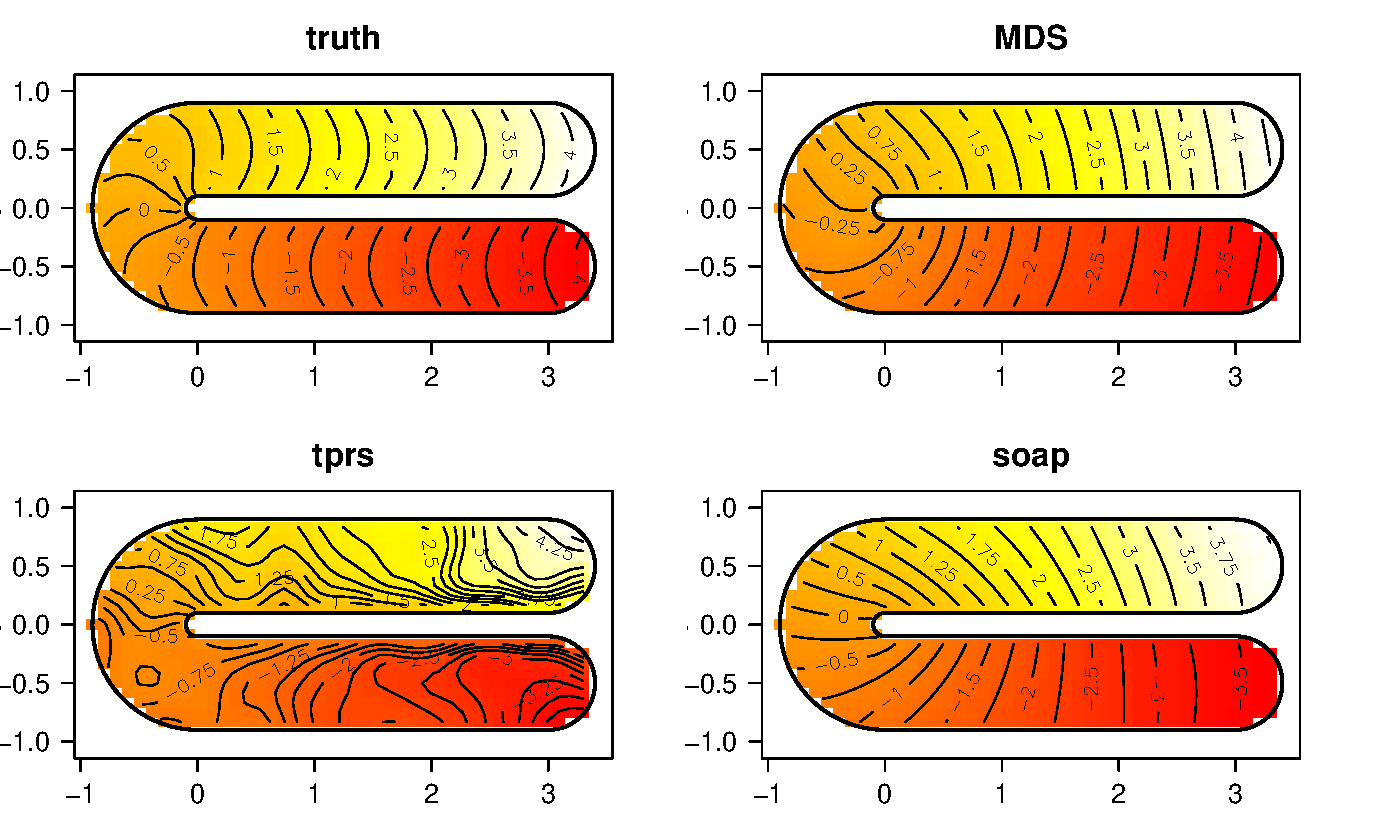
\includegraphics[width=6in]{mds/figs/ramsay-fit-1.pdf} \\
\caption{From top left clockwise: truth for the (modified) Ramsay horseshoe (``truth''), \mdsap\ (``MDS''), the soap film smoother (``soap'') and thin plate splines (``tprs'') when 250 points sampled with noise level set to 1.}
\label{mds-ramsay-fit-1}
% generated (roughly) using ramsay-smooth-test.R
\end{figure}

Just as when the \sch\ transform was used to morph the domain, it is interesting to see what has happened to the distribution of points in space. \Fig{mdsrampoints} shows the effect of the transform on a regular grid of points (left) when they are projected into MDS space (right). The projection has also succeeded in parting the two arms of the horseshoe, reducing leakage (as can be seen in the realisations in \fig{mds-ramsay-fit-1}).

\begin{figure}
\centering
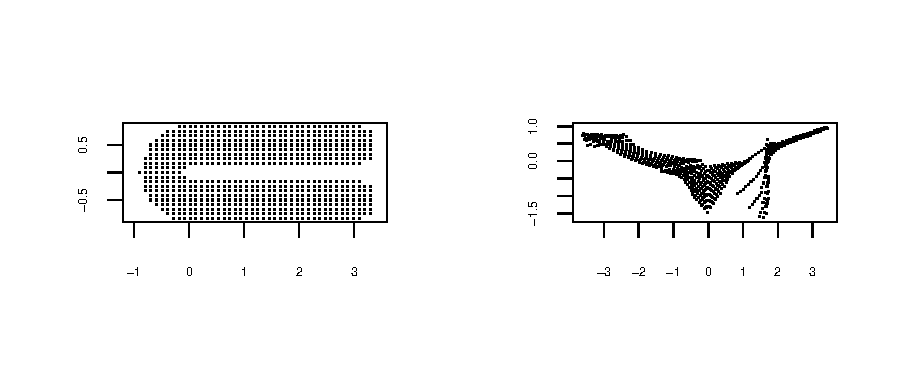
\includegraphics[width=6in]{mds/figs/mdsrampoints.pdf} \\
\caption{A regular grid over the Ramsay horseshoe (left) and its projection into MDS space (right).}
\label{mdsrampoints}
% generated using thesis/mds/figs/mdsrampoints
\end{figure}


\subsection{Peninsula domain}
\label{mds-wt2-sim}

The Ramsay horseshoe is an easy domain to smooth over since it is clear that a transformation should be parting the two arms of the domain. In practise however, there may be ambiguity over which parts of the domain should be separated the most. For this reason a more realistic, complex domain would provide a better insight into the efficacy of the method. The domain shown in \fig{wt2-truth} is an approximation to a coastline with a strong trend along both peninsulae (in a manner similar to that of the horseshoe) but with the added complication of a further peak in the lower right corner.

\subsubsection{Setup}

The simulations consisted of 200 realisations of 250 samples from the surface in \fig{wt2-truth}. Normal noise was added at three levels  0.35, 0.9, and 1.55 (corresponding to signal-to-noise ratios (SNRs) of 0.95, 0.75 and 0.5, respectively. SNRs were calculated as the mean squared correlation between true function value and the truth with error added). Mean squared error over 1253 prediction points (including those points in the sample) was calculated and recorded, along with EDF for each model. The models fitted were:

% wt2 truth 
\begin{figure}
\centering
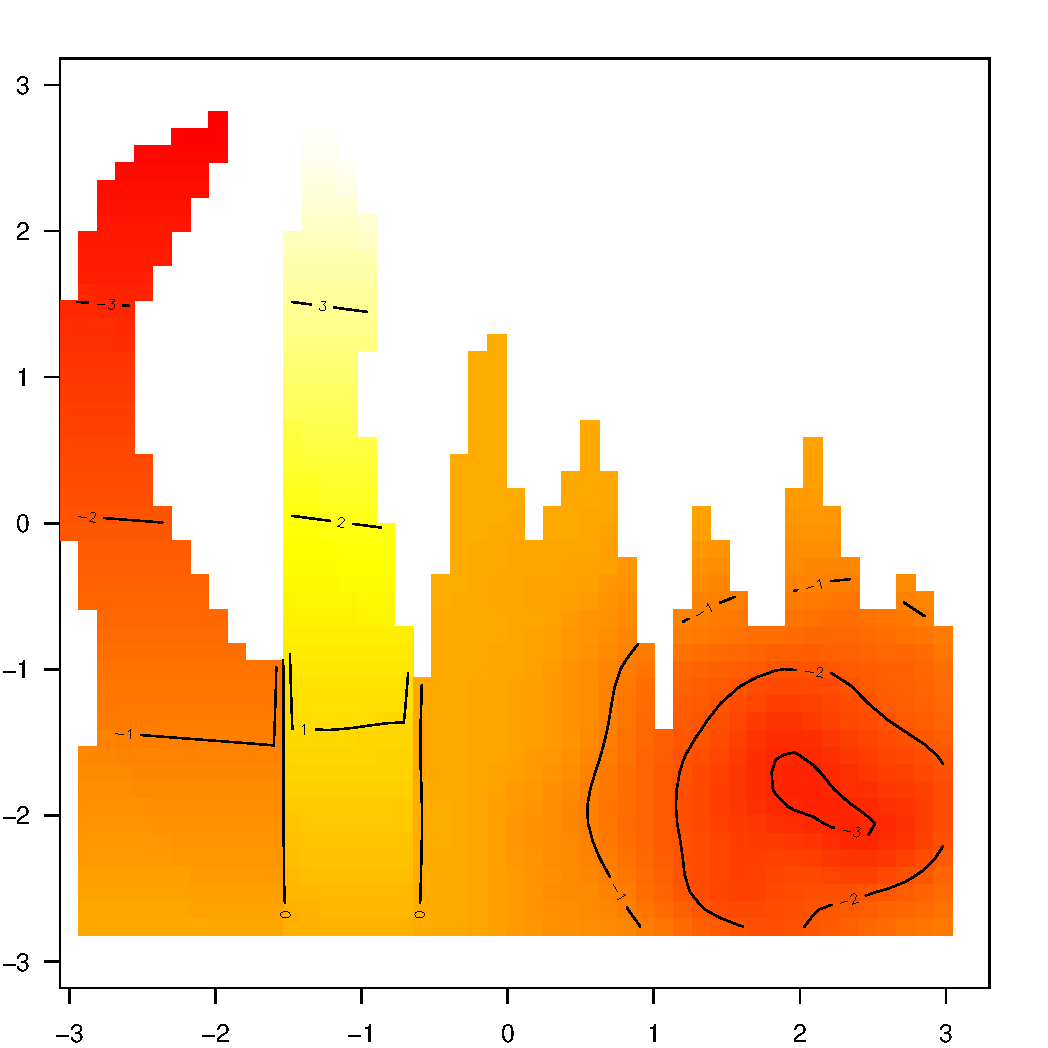
\includegraphics[width=3in]{mds/figs/wt2-truth.pdf} \\
\caption{True function for the domain with multiple peninsulae.}
\label{wt2-truth}
% generated (roughly) using wt2-smooth-test.R
\end{figure}

\begin{enumerate}
\item \emph{Thin plate spline}: bivariate thin plate spline with basis size 100. 
\item \emph{Soap film smoother}: cyclic spline on boundary of basis size 60, 109 internal knots evenly spaced on a grid over the domain.
\item \emph{\mdsap}: after transform a bivariate thin plate spline with basis size 100 was fit. The initial MDS grid was 10 by 10 points square (48 points were inside the domain).
\end{enumerate} 

\subsubsection{Results}

% wt2 fit with error=0.9
\begin{figure}
\centering
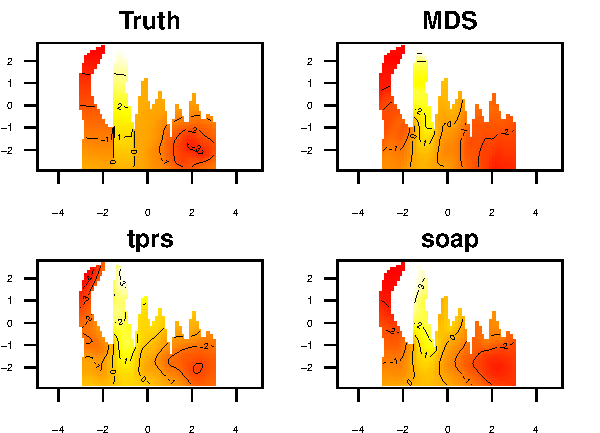
\includegraphics[width=6in]{mds/figs/wt2-comp-09.pdf} \\
\caption{A typical realisation of fits from the multiple peninsulae domain when the noise level is  is set to 0.9 (SNR = 0.75) and sample size is 250. Prediction grid was of size 1253. Clockwise from top left: the true function, prediction from: MDS projection smoothed with \tprs, the soap film smoother and \tprs.}
\label{wt2-comp-0.9}
% generated (roughly) using wt2-smooth-test.R
\end{figure}

Looking at a typical realisation in \fig{wt2-comp-0.9} (noise level = 0.9, SNR = 0.75, sample size 250), the \tprs\ can be seen showing signs on leakage across the two main peninsulae, whereas \mdsap\ and the soap film do not show this. However the \tprs\ does reproduce the peak in the lower right much more faithfully, the other two smoothing over it. In this realisation, \mdsap\ deals with the values inside the peninsula a little better than the soap film smoother (the contour lines are closer to those in the true function). On the other hand, the soap film captures the shape of the lower right peak slightly more accurately.

Figures \ref{mds-wt2-boxplot} and \ref{mds-wt2-boxplot-edf} show boxplots of the MSE and EDF for the models above. There is not a massive difference between the results in MSE terms, the soap film smoother consistently has a statistically significantly lower MSE (at the 0.01 level). The soap film also tends to fit simpler models than the other two approaches except at the highest noise level.

% boxplot for wt2
\begin{figure}
\centering
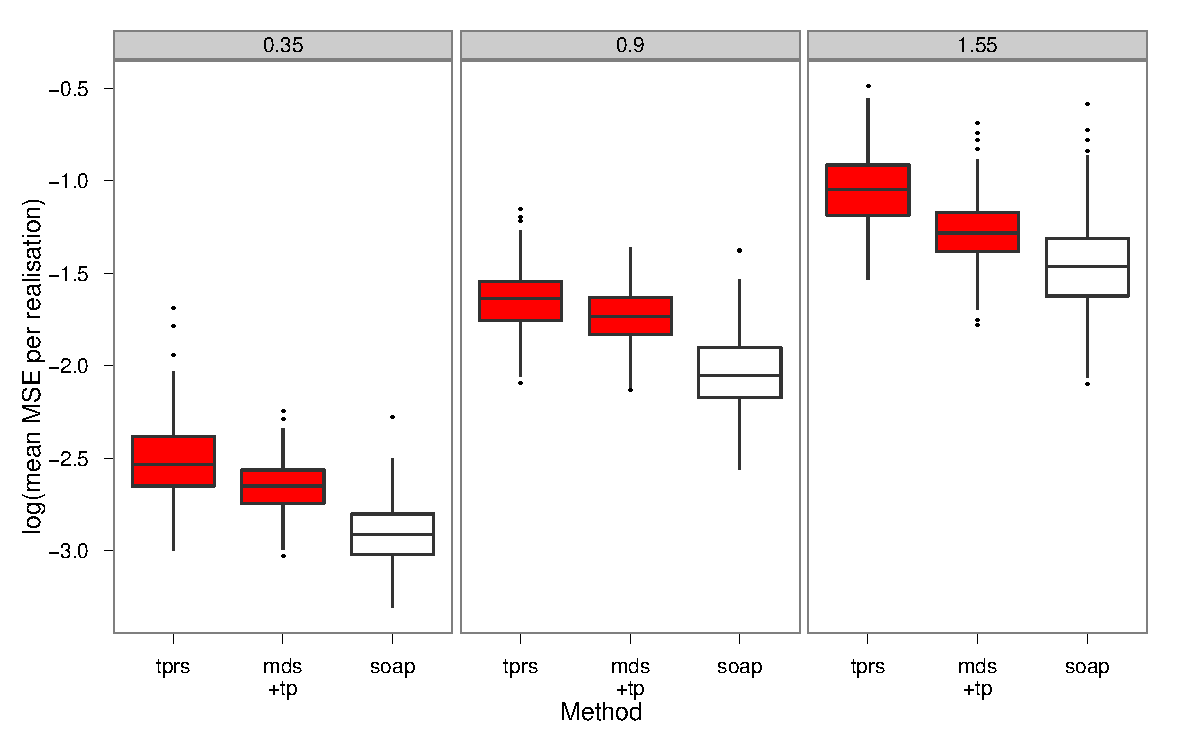
\includegraphics[width=\textwidth]{mds/figs/mds-wt2-boxplot.pdf} \\
\caption{Boxplots of the logarithm of the MSE per realisation of the peninsula domain for the MDS approach (``mds+tp''), soap film smoother (``soap'') and \tprs\ (``tprs'') for noise levels 0.35, 0.9 and 1.55. A paired Wilcoxon signed rank test shows that the MSEs for the two other models were significantly different from the soap film smoother at the 0.01 level.}
\label{mds-wt2-boxplot}
% generated using phd-smoothing/mds/sim/boxplot-wt2-1.R
\end{figure}

% EDF boxplot for wt2
\begin{figure}
\centering
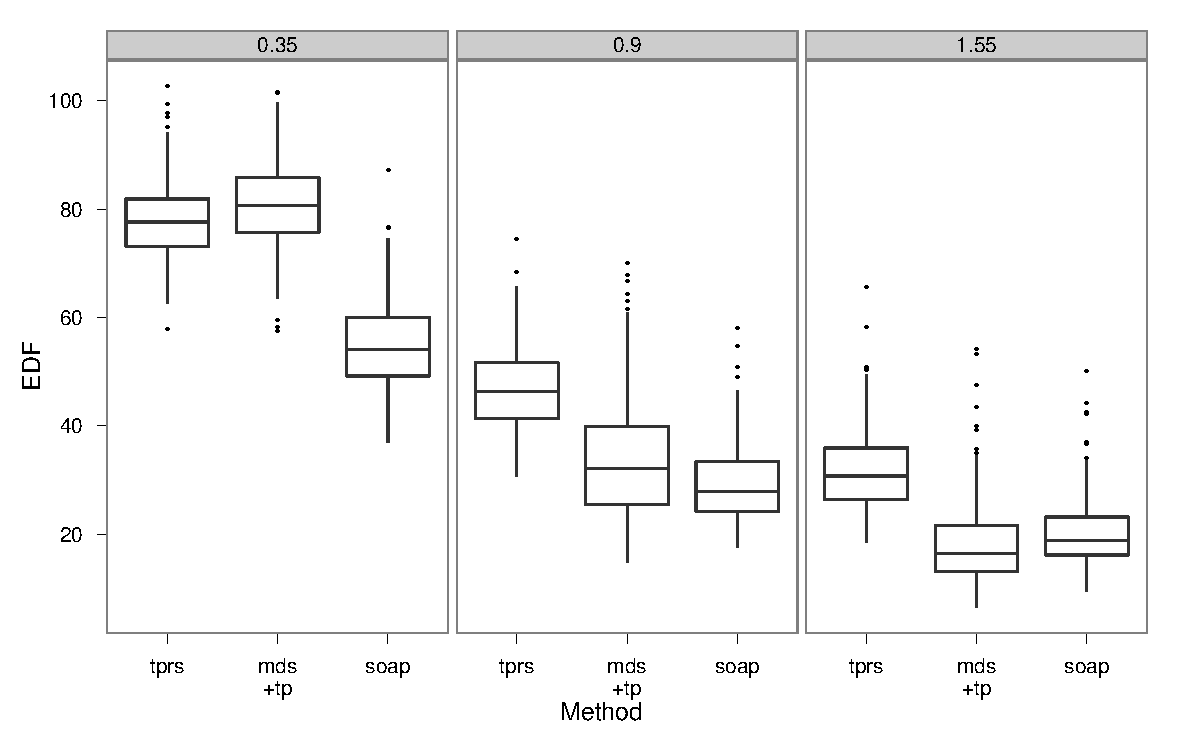
\includegraphics[width=\textwidth]{mds/figs/mds-wt2-boxplot-edf.pdf} \\
\caption{Boxplots of the EDF for each model per realisation of the peninsula domain for the MDS approach(``mds+tp''), soap film smoother (``soap'') and \tprs\ (``tprs'') for noise levels 0.35, 0.9 and 1.55.}
\label{mds-wt2-boxplot-edf}
% generated using phd-smoothing/mds/sim/boxplot-wt2-1-edf.R
\end{figure}


%\begin{table}[t]
%\centering
%\begin{tabular}{c c c c c}
% &  & MSE  & &\\ 
%Noise level & \mdsap & Soap film & Thin plate\\ 
%\hline
%0.35  & 0.07 (0.00062) & 0.0539 (5e-04) &0.082 (0.00104)\\
%0.9  & 0.177 (0.00184) & 0.131 (0.00197) &0.194 (0.00241)\\
%1.55  & 0.286 (0.00438) & 0.236 (0.00434) &0.351 (0.00471)\\
%\end{tabular}
%\begin{tabular}{c c c c c}
% &  & EDF  & &\\ 
%Noise level & \mdsap & Soap film & Thin plate\\ 
%\hline
%0.35 &80.904 (0.571) & 55.698 (0.514) & 77.962 (0.467)\\ 
%0.9 &35.019 (0.764) & 29.717 (0.575) & 48.051 (0.476)\\ 
%1.55 &19.463 (0.573) & 20.292 (0.366) & 32.272 (0.48)\\ 
%\end{tabular}
%\caption{Mean MSE and EDF for the three models fitted to the peninsula domain with standard errors (in brackets) over 200 realisations.}
%\label{wt2resultstable}
%\end{table}

As with the Ramsay horseshoe, it is interesting to see what the projection into MDS space has done to the distribution of the points in the domain. \Fig{wt2-2d-proj} shows points in the domain in Euclidean space and MDS space. There appears to be some high concentrations of points in the far left peninsula and in the right side in the MDS space. This is due to the projection of the points into 2-dimensional space, which can be easily seen in \fig{wt2-3d-proj} where the points have been projected into 3-dimensional space. This shows that there is separation between the smaller peninsulae in higher dimensions that cannot be seen in the 2-dimensional projection.

This high point density in the right side of the MDS space could be the reason for the poor reproduction of the function in that region, seen in \fig{wt2-comp-0.9}. In this portion of space (and in the left peninsula) there is a breakdown in isotropy, which the \tprs\ does not handle well. This must be accounted for in the smooth if accurate models are to be built.

% how the points are projected for wt2
\begin{figure}
\centering
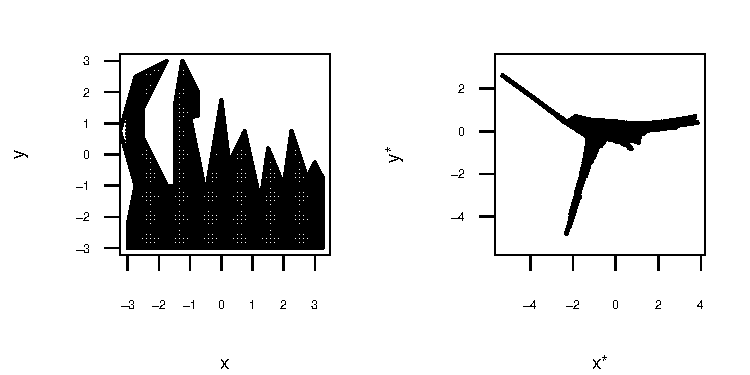
\includegraphics[width=6in]{mds/figs/wt2-2d-proj.pdf} \\
\caption{A regular grid over the peninulae domain (left) and its projection into MDS space (right).}
\label{wt2-2d-proj}
% generated using thesis/mds/figs/wt2-mds.R
\end{figure}

% how the points are projected for wt2 in 3D!
\begin{sidewaysfigure}
\centering
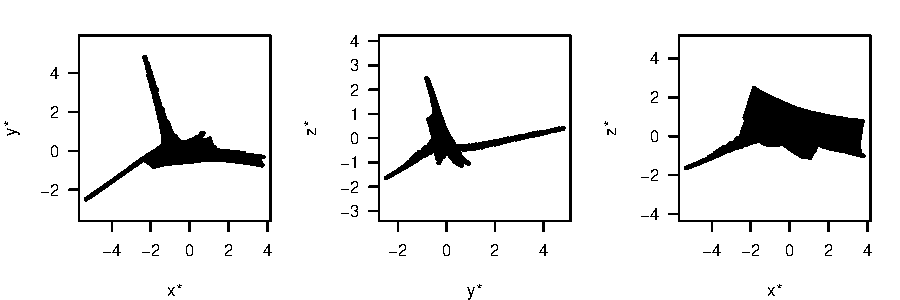
\includegraphics[width=9in]{mds/figs/wt2-3d-proj.pdf} \\
\caption{The peninsula domain projected into 3-dimensional MDS space. The plots show combinations of axes, note that the first panel is the same as the 2-dimensional projection shown in \fig{wt2-2d-proj}.}
\label{wt2-3d-proj}
% generated using thesis/mds/figs/wt2-mds.R
\end{sidewaysfigure}

\subsection{Areas for improvement}

From this set of simulations areas for improvement to \mdsap\ can be seen. First, the above problem of the accuracy of the model (in terms of faithfully reproducing the function) needs to be addressed. Second, running the model is actually quite slow, the calculation of the within-area distances by the algorithm given in \secref{mdsdist} has considerable computational cost, even in comparison to the soap film smoother basis setup. Table \ref{wt2time} shows the average timings for running \mdsap, \tprs\ and soap film smoothers over the peninsula domain

\begin{table}[ht]
\centering
\begin{tabular}{c || c c c c c c}
 & \mdsap & Soap film & Thin plate\\ 
\hline
Fit & 84.852 & 24.678 & 0.402\\ 
Prediction &  53.511 & 29.395 & 0.125\\
\end{tabular}
\label{wt2time}
\caption{Average time (in seconds) to fit and predict on a realisation of the peninsula domain for the three models considered above. Times are averaged over 100 realisations and were found using the elapsed time provided by \textsf{R}'s built-in \texttt{system.time} function. For each realisation a sample of size 250 was taken, then a 1253 values were predicted.}
\end{table}

In order to make \mdsap\ worthwhile for a practitioner to use the method, it would be preferable for it not only to have a sensible physical model, but also outperform the soap film smoother in either (or both) of accuracy and speed.

\section{Making \mdsap\ faster}
\label{mds-faster}

\subsubsection{Calculating MDS by Lanczos iteration}

The \textsf{R} command used to perform the multidimensional scaling, \texttt{cmdscale}, uses the routine \texttt{eigen} in order to perform the requisite matrix eigen-decomposition. This routine will calculate a full eigen-decomposition of the matrix, even if only the first $k$ eigenvalues and/or eigenvectors are required. Using Lanczos iteration, only the first $k$ eigenvalues (in numeric or algebraic size order) will be calculated.

The  Lanczos procedure works by iteratively building a symmetric $i\cross i$ tridiagonal matrix (at the $i^{\text{th}}$ iteration) which has eigenvalues approximately the same as the $i$ largest eigenvalues of the original matrix. Further detail is given in \citeb{simonbook}, pp. 335-337.

The \texttt{igraph} library for \textsf{R} provides an interface to the C++ package \texttt{ARPACK++} which implements the Lanczos procedure. Replacing the \texttt{cmdscale} command with one that uses the \texttt{ARPACK++} interface provided by \texttt{igraph} will decrease the number of computations needed, thus making the calculation of the eigenvalues and vectors faster.

A quick benchmark shows that \texttt{ARPACK++} can compute the first two eigenvalues and vectors faster than just using \texttt{eigen} when the eigen-decomposition to be computed is of a large matrix. Generating a 1000 by 1000 symmetric matrix of normal random deviates with mean 0 and variance 1000, then performing an eigen-decomposition takes 1.68 seconds using \texttt{ARPACK++} and 3.26 seconds using \texttt{eigen} (averaged over 100 runs). This advantage drops once the matrix is around 100 by 100 and the cost of calling the C++ code begins to dominate; in this case \texttt{ARPACK++} takes 0.037 seconds and \texttt{eigen} takes 0.034 (averaged over 100 runs). Given that the disadvantage is in the order of hundredths of a second and the advantage is a two-fold decrease in computational time, it makes sense to use the \texttt{ARPACK++} code in all cases.

% sim code is at ~/phd-smoothing/mds/lanczos/time-arpack.R

\subsubsection{Partial path calculation}

Many of the distances stored in $\mathbf{D}$ are calculated by simply using the Euclidean metric since for the corresponding point pairs, there is no part of the path between them that lies outside of the domain. It is often the case that the paths that need to be calculated are on a grid (for example, when doing prediction). This leads us to believe that there are many sets of paths that are rather similar. These paths may perhaps only differ in their final vertex. Given that, in this case, there is a lot of wasted computational time spent calculating similar paths, it would be useful to exploit this problem, and use it to increase the speed of the path calculation.

The idea here is to use a sparse grid to first calculate a set of paths that are then saved. These saved paths then form the base of the other paths that need to be calculated. Finally, these paths are optimised in the same manner as the algorithm given in \secref{mdsdist}. This removes the expensive calculation in the middle of the path, where perhaps the bulk of the interactions with the boundary take place.

The algorithm is as follows, with notation and routines (INIT, DELETE, ALTER and ITER) identical to those in \secref{mdsdist}. 

Again, taking points $p_i$ and $p_j$ in the set of points in the domain that we wish to find the shortest paths for and drawing a path between them, finding within-area distance with respect to the boundary of $\Gamma$.

\begin{enumerate}
 \item Begin by creating a sparse grid of within $\Gamma$ and calculate the ($M$, say) non-Euclidean within-area paths between all pairs of points exactly as in \secref{mdsdist}. Store these paths as $\mathcal{P}_1,\ldots, \mathcal{P}_M$.
\item For each unique pairing of $p_i$ and $p_j$ in the full data set, calculate the path using one of the following:
	\begin{enumerate}
	\item Find a $\mathcal{P}_k$ such that the path between $p_i$ and one end of $\mathcal{P}_k$ and $p_j$ and the other end of $\mathcal{P}_k$ is Euclidean within $\Gamma$. Join $p_i$ and $p_j$ onto the appropriate ends of $\mathcal{P}_k$ and run ITER (ie. alternate between DELETE and ALTER) until convergence.
	\item If there is no Euclidean path between $p_i$ and $p_j$, and no $\mathcal{P}_k$ can be found, then calculate the path between $p_i$ and $p_j$ as in \secref{mdsdist}. 
	\end{enumerate}
\end{enumerate}

Note that those paths between points in the sparse grid which are Euclidean are not stored since it is always at least as expensive to store, add and optimise those paths then calculating them from scratch. If the path we want to calculate is Euclidean anyway, then retrieving a Euclidean path, adding in $p_i$ and $p_j$, and then iterating over ALTER and DELETE steps to make it both the shortest and a Euclidean path will take longer than just creating a Euclidean path to begin with. If the path between $p_i$ and $p_j$ is non-Euclidean then the non-Euclidean part of the path must lie outside $\mathcal{P}_k$ (by definition) and therefore will take the same number of operations to find the boundary crossing points and calculate the shortest path around the feature locally as it will to calculating the whole path from scratch.


\subsubsection{Simulation - Lanczos and partial path calculation improvements}

Taking both the Lanczos procedure and the partial path calculation together, a simulation was run to find the improvements in terms of computational time for the double peninsulae domain. Average time for both model fitting and prediction are given in \tabref{wt2itime} for 100 realisations. 

The differences between the first two columns are striking. The partial path calculation has dramatically reduced the computational time for the calculation of the entries of the distance matrix, making it faster than the soap film smoother for the model fitting, and reducing the prediction time to a third of its previous value. The \tprs\ times are shown to give a comparison for the time actually taken to fit the model, the remaining time for \mdsap\ is taken up by calculating the distances and performing the MDS.

\begin{table}[ht]
\centering
\begin{tabular}{c || c c c c c c}
%  no speedup           speedup
 & \mdsap & \mdsap (\textit{pp}) & Soap film & Thin plate\\ 
\hline
Fit & 84.852 & 18.653 & 24.678 & 0.402\\ 
Prediction & 155.400 & 53.511 & 29.395 & 0.125\\
\end{tabular}
\label{wt2itime}
\caption{Average time (in seconds) to fit and predict on a realisation of the peninsula domain for the three models considered above. Times are averaged over 100 realisations and were found using the elapsed time provided by \textsf{R}'s built-in \texttt{system.time} function. For each realisation a sample of size 250 was taken, then a 1253 values were predicted. For the \mdsap\ columns \textit{pp} indicates the cases where the partial paths were pre-calculated, those not marked use the algorithm given in \secref{mdsdist}.}
\end{table}


\section{Using penalty adjustments to correct for\\ squashing}
\label{mds-penadjust}

Figures \ref{wt2-2d-proj} and \ref{wt2-3d-proj} show that the points in the peninsulae domain have been squashed together in some areas. In particular, this occurs in the peninsulae themselves. Since the motivation here is to improve estimates in the peninsulae, it would be extremely unfortunate if the transformation was detrimental to the smoother's performance in these areas (albeit in a different way than was originally problematic). The squashing is similar to that seen in \secref{sch-crowding} when the \sch\ transform was used to transform the domain, although not as severe as the crowding seen there, this can still be problematic (as was seen in \secref{sc-penin}). 

Uneven point density can cause problems for the smoother since the measure of smoothness will change.  Squashing space together may make the data appear more variable than it in fact is (see figure \ref{1dadjust} for a 1-dimensional example). Moving into two dimensions, an isotropic smooth seems like an unrealistic choice if the point densities are different in each dimension. One might expect that the amount of smoothing required would be a function of the density of points at that location.

The higher MSEs shown in figure \ref{mds-wt2-boxplot} might be explained by the change in density of points in the domain after it has been transformed into MDS space. In this case adjusting the thin plate spline penalty in order to take into account the change in point density in MDS space might improve performance.

An alternative approach would be to use a tensor product basis (of, for example, P-splines as was used in \secref{sc-sims}) where there is a separate smoothing parameter for each dimension. However, thin plate splines have other appealing properties (in particular the eigen-based approach of \cite{wood2003}, to avoid knot placement issues). A tensor product smooth may also still run into problems in each dimension with regard to the squashing of space. For these reasons, this section explores the utility of penalty adjustments based on point density for thin plate splines.

\subsection{Overview}

\citeb{wood2000} shows that given some transform of a variable, $x_2$ say, such that $x_{2i}^\prime=x_{2i}/k$, then $f(x_1,x_2^\prime k)$ will give the same fit as $f(x_1,x_2)$ (ie. the fit will be the same under the new coordinates), if the penalty is changed to:
\begin{equation}
\int\int_\mathbb{R}^2 \left ( \frac{\partial^2 f}{\partial x_1^2} \right )^2 + 2k\left ( \frac{\partial^2 f}{\partial x_1 \partial x_2} \right )^2 + k^3\left ( \frac{\partial^2 f}{\partial x_2^2} \right )^2 \text{d}x_1 \text{d}x_2,
\label{adjustedintegral}
\end{equation}
from the usual \tprs\ penalty (see \secref{GAMtprspenalty}).

This approach will only handle a linear rescaling in one dimension; in the case of the MDS distortions, non-linear re-scalings in two dimensions must be addressed. To generalise \eqn{adjustedintegral} to the non-linear two-dimensional case a function must be found, $\mathcal{L}^*(x_1,x_2)$ say, which evaluates to the change in density for each point in the domain. 

Such a function should allow the smoothness to be adapted according to the degree to which space has been squashed, thus getting around the spatial heterogeneity which appears to be affecting the model. The calculation of $\mathcal{L}^*(x_1,x_2)$ is elaborated on below.

Given that the function $\mathcal{L}^*(x_1,x_2)$ is known, the penalty is given as:
\begin{equation}
\int\int_{\Gamma^\prime} \mathcal{L}^*(x_1,x_2) \left \{ \left (\frac{\partial^2 f(x_1,x_2)}{\partial x_1^2}\right )^2 + 2\left (\frac{\partial^2 f(x_1,x_2)}{\partial x_1 \partial x_2}\right )^2 + \left (\frac{\partial^2 f(x_1,x_2)}{\partial x_2^2}\right )^2\right \} \text{d}x_1 \text{d}x_2.
\label{kdeadjust}
\end{equation}
Note the change of integration domain from $\mathbb{R}^2$ to $\Gamma^\prime$ (the transformed domain), as well as the pre-multiplication by the density function.

Before moving straight to the 2-dimensional case above, the method was tested in one dimension.

\subsection{Penalty adjustments in one dimension}

Before implementing this approach in full a a test was run in one dimension. The function:
\be
g(x)=0.2x^{11}\left \{ 10(1-x) \right \}^6+10(10x)^3(1-x)^{10},
\label{hardfcn}
\ee
was used and contracted by factors of $20,1,0.05,1$ over the regions $[0,0.4]$, $(0.4,0.6]$, $(0.6,0.8]$ and $(0.8,1]$, respectively. The function and its squashed form are shown in the top left and right panels (respectively) of \fig{1dadjust}. Evaluating 100, equally spaced, points over the interval $[0,1]$ using a \tprs\ and then predicting back onto the same points yielded the blue lines in the lower two plots. The left of these shows the prediction in the transformed space and the right in the original space. The green line was produced using a \tprs\ with the adjusted penalty matrix. As can be seen from the plot, the fit has been improved greatly, but how is the adjustment calculated?

% 1d adjustment 2x2 diagram
\begin{figure}
\centering
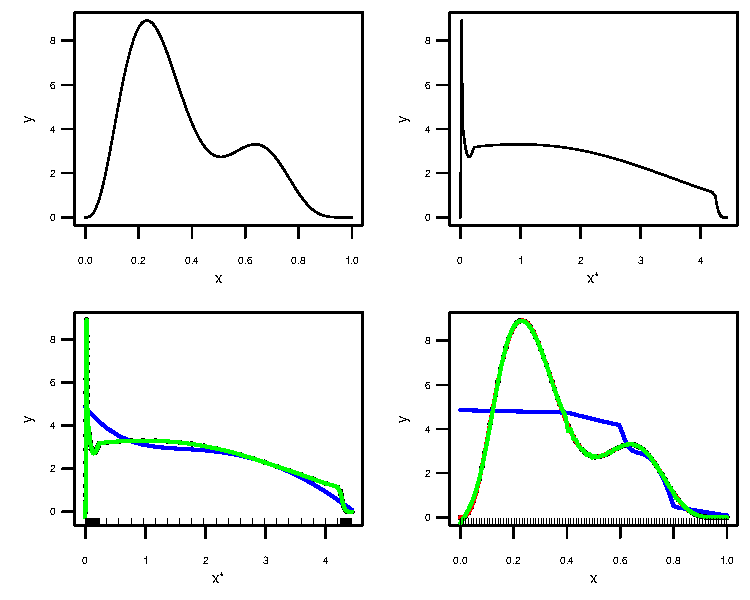
\includegraphics[width=6in]{mds/figs/1dadjust.pdf} \\
\caption{Using penalty adjustments to fit a regression spline to \eqn{hardfcn} after it has been squashed. The function in the top left is squashed to the form in the top right. The bottom left plot shows the fit from a \tprs\ (blue) and a \tprs\ with adjusted penalty (green) in the transformed space. The bottom right shows the same fit in the untransformed space. Clearly, the penalty adjustment improves the fit.}
\label{1dadjust}
% generated by thesis/mds/figs/tpintexp.R
\end{figure}

\subsubsection{Penalty adjustment calculation}

For the moment let us take $f$ to be a one dimensional smooth function. It may be decomposed into its basis functions and coefficients as seen in (\ref{intro-basisdecomp}):
\begin{equation*}
\hat{f}(x)=\sum_{j=1}^J \hat{\beta}_j b_j(x).
\end{equation*}
The $ij^\text{th}$ element of the penalty matrix (see \secref{GAMpenalties}) is then given as:
\begin{equation*}
\mathbf{S}_{ij}= \int_a^b \mathcal{L}^*(x) \frac{\partial^2 b_i(x)}{\partial x^2}\frac{\partial^2 b_j(x)}{\partial x^2} \text{d}x = \int_a^b \mathcal{L}^*(x) b^{\prime\prime}_i(x) b^{\prime\prime}_j(x) \text{d}x,
\end{equation*}
in one dimension (letting a prime indicate differentiation with respect to $x$). The integral can then be approximated by the midpoint rule as:
\begin{equation}
\mathbf{S}_{ij}= \frac{b-a}{K}\sum_{k=1}^K \mathcal{L}^*(x_k) b^{\prime\prime}_i(x_k) b^{\prime\prime}_j(x_k) \quad \text{for} \quad x_k=a+\frac{(k-0.5)(b-a)}{K},
\label{midpointS}
\end{equation}
for $k=1,\dots, K$. Second derivatives are evaluated by finite differences in the usual manner:
\begin{equation}
\label{bfinitediff}
b^{\prime\prime}_i(x) = \frac{ b_i(x+2\epsilon) - 2b_i(x+\epsilon) + b_i(x)}{\epsilon^2}.
\end{equation}
For the sake of efficiency, a $K\cross J$ matrix, $\mathbf{D}$, is calculated with $kj^\text{th}$ element:
\begin{equation}
\mathbf{D}_{kj}=\sqrt{\mathcal{L}^*(x_k)} b^{\prime\prime}_j(x_k),
\label{oneDD}
\end{equation}
for $x_k$ as above. Then $\mathbf{S}$ may be calculated as:
\begin{equation*}
\mathbf{S}=\frac{b-a}{K}\tr{\mathbf{D}}\mathbf{D}.
\end{equation*}

In this example $\mathcal{L}^*(x)$ was simply calculated using the inverse of the cube of the factor by which the relevant part of the domain (given above) was squashed. 

\subsubsection{Checking that the adjustment works}

\Fig{1dadjust} shows that the adjustment faithfully repdroduces $g(x)$ for the zero error case, fitting a much more sensible model than the standard \tprs. To check that this is true more generally, $\lambda$ was specified (rather than being automatically selected) so that the models with modified and unmodified penalties would have the same EDF. \Fig{1dedfdia} shows such an experiment. Using \eqn{hardfcn} with standard normal noise (multiplied by 0.4) added the smoothing parameter was set so that the EDF would be 71, 19 and 42 (working down the diagram). The plots show that the adjustment deviates from truth at most as badly as the vanilla \tprs\ but overall corrects some of the departures from the truth, even in presence of error with a restricted basis.

% 1d adjustment EDF comparison diagram
\begin{figure}
\centering
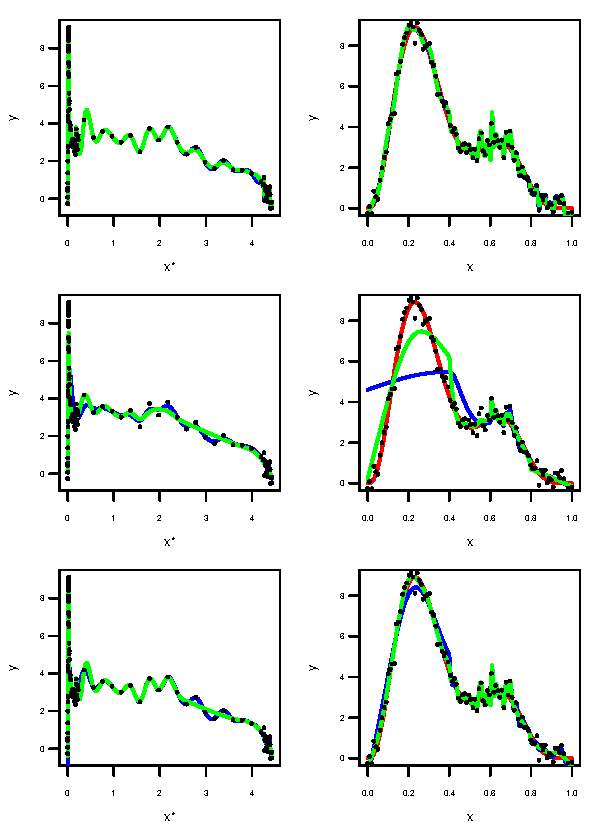
\includegraphics[width=5.5in]{mds/figs/1dedfdia.pdf} \\
\caption{Predictions in transformed and untransformed (left and right columns respectively) for \tprs\ (blue line) and penalty adjusted \tprs\ (green line) fits to the function in \eqn{hardfcn} when the smoothing parameter was pre set to give EDF of 71, 19, and 42 (top to bottom).}
\label{1dedfdia}
% generated by thesis/mds/figs/tpintexp.R
\end{figure}


\subsection{Penalty adjustments in two dimensions}

Using a similar procedures as for one dimension, the two dimensional case can be addressed. Again looking at the $ij^\text{th}$ element of $\mathbf{S}$, for the two dimensional case we have:
\begin{align*}
\mathbf{S}_{ij}= \int\int_{\Gamma^\prime} \mathcal{L}^*(x_1,x_2) \Bigg ( & \frac{\partial^2 b_i(x_1,x_2)}{\partial x_1^2}\frac{\partial^2 b_j(x_1,x_2)}{\partial x_1^2}+2\frac{\partial^2 b_i(x_1,x_2)}{\partial x_1 \partial x_2}\frac{\partial^2 b_j(x_1,x_2)}{\partial x_1 \partial x_2}+ \\ 
& \frac{\partial^2 b_i(x_1,x_2)}{\partial x_2^2}\frac{\partial^2 b_j(x_1,x_2)}{\partial x_2^2} \Bigg )  \text{d}x_1\text{d}x_2.
\end{align*}
Matrices analogous to \eqn{oneDD} can be constructed using the finite differences from \eqn{bfinitediff} for differentials $x_1$ and $x_2$ individually and
\begin{equation*}
\frac{\partial^2 b_i(x_1,x_2)}{\partial x_1 \partial x_2} = \frac{ b_i(x_1+\epsilon,x_2+\epsilon) - b_i(x_1+\epsilon,x_2) - b_i(x_1,x_2+\epsilon) + b_i(x_1,x_2)}{\epsilon^2},
\end{equation*}
for the cross term. The matrices then take the form:
\begin{equation*}
[\mathbf{D}_{x_1}]_{kj}=\sqrt{\mathcal{L}^*(x_{1k},x_{2k})} \frac{\partial^2 b_j(x_{1k},x_{2k})}{\partial x_1^2},
\end{equation*}
\begin{equation*}
[\mathbf{D}_{x_2}]_{kj}=\sqrt{\mathcal{L}^*(x_{1k},x_{2k})} \frac{\partial^2 b_j(x_{1k},x_{2k})}{\partial x_2^2},
\end{equation*}
\begin{equation*}
[\mathbf{D}_{x_1 x_2}]_{kj}=\sqrt{\mathcal{L}^*(x_{1k},x_{2k})} \frac{\partial^2 b_j(x_{1k},x_{2k})}{\partial x_1 \partial x_2}.
\end{equation*}
So we may then express $\mathbf{S}$ as:
\begin{equation*}
\mathbf{S}=\tr{\mathbf{D}_{x_1}}\mathbf{D}_{x_1} + \tr{\mathbf{D}_{x_1 x_2}}\mathbf{D}_{x_1 x_2} + \tr{\mathbf{D}_{x_2}}\mathbf{D}_{x_2}.
\end{equation*}
Where the partial derivative evaluation points ($x_{1k}$ and $x_{2k}$) now form a grid for the integration to be calculated. First defining $x^\dagger_{1k}$ and $x^\dagger_{2k}$ analogously to \ref{midpointS}, we have:
\begin{equation*}
x^\dagger_{1k}=a_{x_1}+\frac{(k-0.5)(b_{x_1}-a_{x_1})}{K},\quad
x^\dagger_{2k}=a_{x_2}+\frac{(k-0.5)(b_{x_2}-a_{x_2})}{K},
\end{equation*}
for $k=1,\dots,K$. The integration grid may then be constructed as:
\begin{equation*}
\left \{x_{1k} : k=1,\dots,K \right \} = \left \{x^\dagger_{11},x^\dagger_{11},x^\dagger_{11},\dots, x^\dagger_{12}, x^\dagger_{12}, x^\dagger_{12},\dots, x^\dagger_{1K}, x^\dagger_{1K}, x^\dagger_{1K}\right \},
\end{equation*}
\begin{equation*}
\left \{x_{2k} : k=1,\dots,K \right \} = \left \{x^\dagger_{11},x^\dagger_{22}, x^\dagger_{23},\dots, x^\dagger_{2K},x^\dagger_{11},x^\dagger_{22}, x^\dagger_{23},\dots, x^\dagger_{2K},\dots\right \}.
\end{equation*}
Finally, those $(x_{1k},x_{2k})$ that do not lie inside the boundary in MDS space are removed leaving only those points that lie inside (so that the integration is performed over $\Gamma^\prime$).

\subsubsection{Finding $\mathcal{L}^*$}

Calculating $\mathcal{L}^*(x_1,x_2)$ in two dimensions is more tricky than in the one dimensional case. Since the two-dimensional case is to be used in practise, the method for finding $\mathcal{L}^*(x_1,x_2)$ must depend on the MDS configuration, as the stretch factors will not be known \emph{a priori} (as was the case in the previous example).

The general idea is to make $\mathcal{L}^*(x_1,x_2)$ a function of the change in density of points caused by projecting the original space into MDS space. However, if we assume that the density in the untransformed space is $1$ everywhere, we merely need to calculate the density in MDS space. Having calculated the point density in MDS space, $\mathcal{L}^*(x_1,x_2)$ is just some function of this density.

In order to find calculate the point density in MDS space, the following steps are performed:

\begin{enumerate}
\item A grid in the original space is mapped into the MDS space. Ideally, this grid would be dense enough for it to be possible to just count the number transformed points in each square of a regular mesh. However, it would be computationally demanding to project a dense grid into MDS space, so instead a sparse grid is used and then interpolated. This consisted of taking 10 equally spaced points on each side of the square and drawing lines between points on opposing sides. Where the lines crossed were the extra points (along with those points lying on the boundary of the square itself).
\item The interpolated points are then used to estimate the overall point density in MDS space by simply counting the number of points there were in each of a set of squares made from the integration grid, call is $\mathcal{L}(x_1,x_2)$. This is shown in \fig{densgrid} for the double peninsulae domain. 
\item Then define $\mathcal{L}^*(x,y)$ as the function
\begin{equation*}
\mathcal{L}^*(x_1,x_2)=\frac{1}{ \left \{ 1+\mathcal{L}(x_1,x_2) \right \}^{3/2}}.
\end{equation*}
The $+1$ in the denominator avoids division by zero when evaluating $\mathcal{L}^*(x_1,x_2)$. The fact that $\mathcal{L}^*(x_1,x_2)$ is then a piecewise function should not be too worrying since the aim here is to address the broader problems with the change in spatial density, not the fine-gained details.
\end{enumerate}

Note that the power is now $\frac{3}{2}$. This is since we do not know the contraction/expansion in each direction individually, but rather the overall change in area. As such we use $\frac{3}{2}$ rather than the cubic on $x$ and $y$ and unitary on the cross term. Several other options were also tested (including changing the power and $+1$ in the denominator) however it was found that the above formulation worked best and so only those results are shown here.

\begin{figure}
\centering
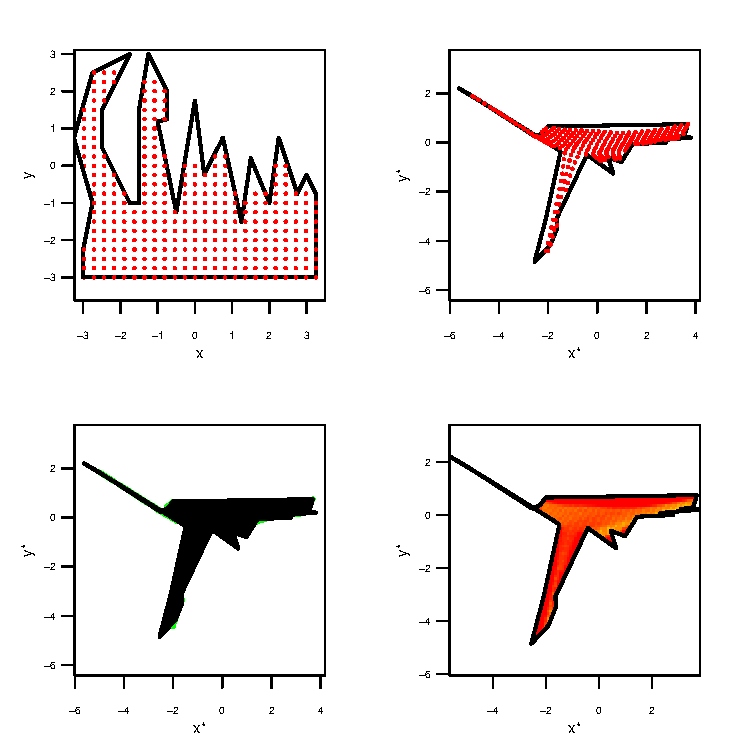
\includegraphics{mds/figs/densgrid.pdf} \\
\caption{The grids used to calculate $\mathcal{L}^*(x_1,x_2)$ for the double peninsulae domain. The red grid in the top left figure is mapped to the red grid in the top right panel. The red points in the top right are then used as the basis for the interpolation in the bottom left. The number of green points in each of the squares made from the black points in the bottom left plot are used to calculate the spatial density in that square. The heat map in the bottom right shows the values of $\mathcal{L}(x_1,x_2)$ (i.e. the density of the green points), here red is low density, yellow is high. Note that some of the points lie outside of the boundary in the MDS projections. This is due to the boundary in MDS space being the straight line interpolant of the vertices of the boundary in the original space.}
\label{densgrid}
% generated by phd-smoothing/mds/wt2-intexp.R and intexp/smooth2.c.R with comments removed
\end{figure}

\subsubsection{Checking that the adjustment works}

In order to make sure that the adjustment works in both the known and unknown contraction/expansion case, a small simulation was run. In this case a surface consisting of two bivariate normal distributions (mean vectors $(0,-0.5)$ and $(0,0.5)$, covariance matrix diagonal entries $(0.2,0.1)$) were sampled from (sample size 300) and then noise added from a $\text{normal}(0,0.05)$ distribution. The surface was then divided into its four constituent quadrants about the origin and squashed according to the following factors (in $(x_1,x_2)$ pairs, in order top left, top right, bottom left, bottom right): ((0.3,5), (1,5), (0.3,1), (1,1)).

The samples were then used to fit a standard \tprs\ model, \tprs\ with adjusted penalty with known stretch factors and a \tprs\ with $\mathcal{L}^*(x_1,x_2)$ estimated from the data. The mean squared error between the truth and prediction over a dense (50 by 50) grid was then calculated.

The simulation results show that there is a decrease in MSE when the expansion/contraction of the space is taken into account (MSEs were: $2.355, 2.300 \text{ and } 2.305$ for thin plate regression splines, known stretch and estimated stretch, respectively). Unfortunately this didn't offer the same visual improvement as the 1-dimensional case.

The next section puts the adjusted penalty approach to the test on the peninsulae domain seen previously and the chlorophyll levels data set seen in the introduction.

\subsection{Wider simulations and real data}

\subsubsection{Peninsulae domain}
\label{wt2bigsim}

Using the same setup as in \secref{mds-wt2-sim}, for each error level (0.35, 0.9, and 1.55), 200 realisations were generated. From these 250 samples were drawn to fit the model, predictions were made over a grid of 1253 points with MSE and EDF recorded per model for each simulation. 

The models that were fitted were:
\begin{enumerate}
\item \emph{tprs}: \tprs\ with basis size 140.
\item \emph{mds+tp}: \mdsap\ using a \tprs\ with basis size 140.
\item \emph{mds 3D}: \mdsap\ using a 3-dimensional \tprs\ with basis size 140. Here MDS was used to project the data into three dimensions rather than two.
\item \emph{mds+adj}: \mdsap\ using a \tprs\ with basis size 140, with penalty adjustments.
\item \emph{soap}: soap film smoother using 109 internal knots evenly spaced on a grid over the domain, with boundary basis size 60.
\end{enumerate}

The results from mds+adj are actually worse than those from just mds+tp in all but the lowest noise case. \Fig{big-wt2-mses} shows boxplots of these results.

However, all is not lost, MDS+3D seems competitive across the board, but is always significantly worse than the soap film smoother (by a paired Wilcoxon signed rank test on the MSEs).  As for the 3-dimensional projection, the plots in \fig{wt2-3d-proj} show that the additional dimension allows for further separation of both a large and small peninsulae, which should help with the anisotropy as well as leakage. As would be expected, the method using the adjusted penalty had a lower EDF than the other methods aside from the vanilla thin plate splines (see figure \ref{big-wt2-edfs}). Interestingly the model using the 3-dimensional projection also has a low EDF, showing that there may be some utility in using such a method especially considering its relatively low MSE.

A Wilcoxon signed rank test, matching pairs between realisations showed that there was a significant difference between the MSE of each model and the soap film smoother. As can be seen from \fig{big-wt2-mses}, soap outperforms all of the other methods on this domain, with MDS+3D coming in second. 

Finally, note that there were three realisations omitted (for all models) in figures \ref{big-wt2-mses} and \ref{big-wt2-edfs}. In these realisations the soap film smoother failed to fit the model due to knot placement. These can be safely removed as, in practise, the computer would inform the user that the knot placement was not appropriate and the knot layout could be altered.

%\begin{sidewaystable}[p]
%\centering
%\begin{tabular}{c c c c c c}
% & &  MSE  & & &\\ 
%Noise level  & tprs & mds+tp & mds+tp 3D & mds+tp+adj & soap\\ 
%\hline
%0.35  & 0.0832 (1e-04) & 0.0713 (5e-05) &  0.0579 (5e-05) & 0.0697 (5e-05) & 0.0598 (0.00032) \\ 
%0.9  & 0.1957 (0.00017) & 0.1788 (0.00013) & 0.1478 (0.00014) & 0.1875 (0.00017) & 0.1616 (0.00201) \\ 
%1.55  & 0.3576 (0.00035) & 0.285 (0.00027) & 0.2765 (0.00032) & 0.3509 (4e-04) & 0.245 (0.00034) \\
%\end{tabular}
%\begin{tabular}{c c c c c c}
% & &  EDF  & & &\\ 
%Noise level  & tprs & mds+tp & mds+tp 3D & mds+tp+adj & soap\\ 
%\hline
%0.35  & 77.8675 (0.03803) & 80.5454 (0.04111) & 61.3458 (0.05324) & 73.3275 (0.03707) & 55.2464 (0.04684)\\ 
%0.9  & 47.0214 (0.0378) & 34.357 (0.05645)  & 30.5807 (0.04027) & 40.409 (0.03805) & 29.6874 (0.04514) \\
%1.55  & 31.8803 (0.03843) & 18.3575 (0.03865) & 19.7871 (0.03128) & 26.6778 (0.03572) & 20.3529 (0.03171)\\ 
%\end{tabular}
%\caption{Mean MSE and EDF for the five models fitted to the peninsula domain with standard errors (in brackets) over 197 realisations.}
%\label{bigwt2resultstable}
%\end{sidewaystable}

% big wt2 sim MSEs
\begin{figure}
\centering
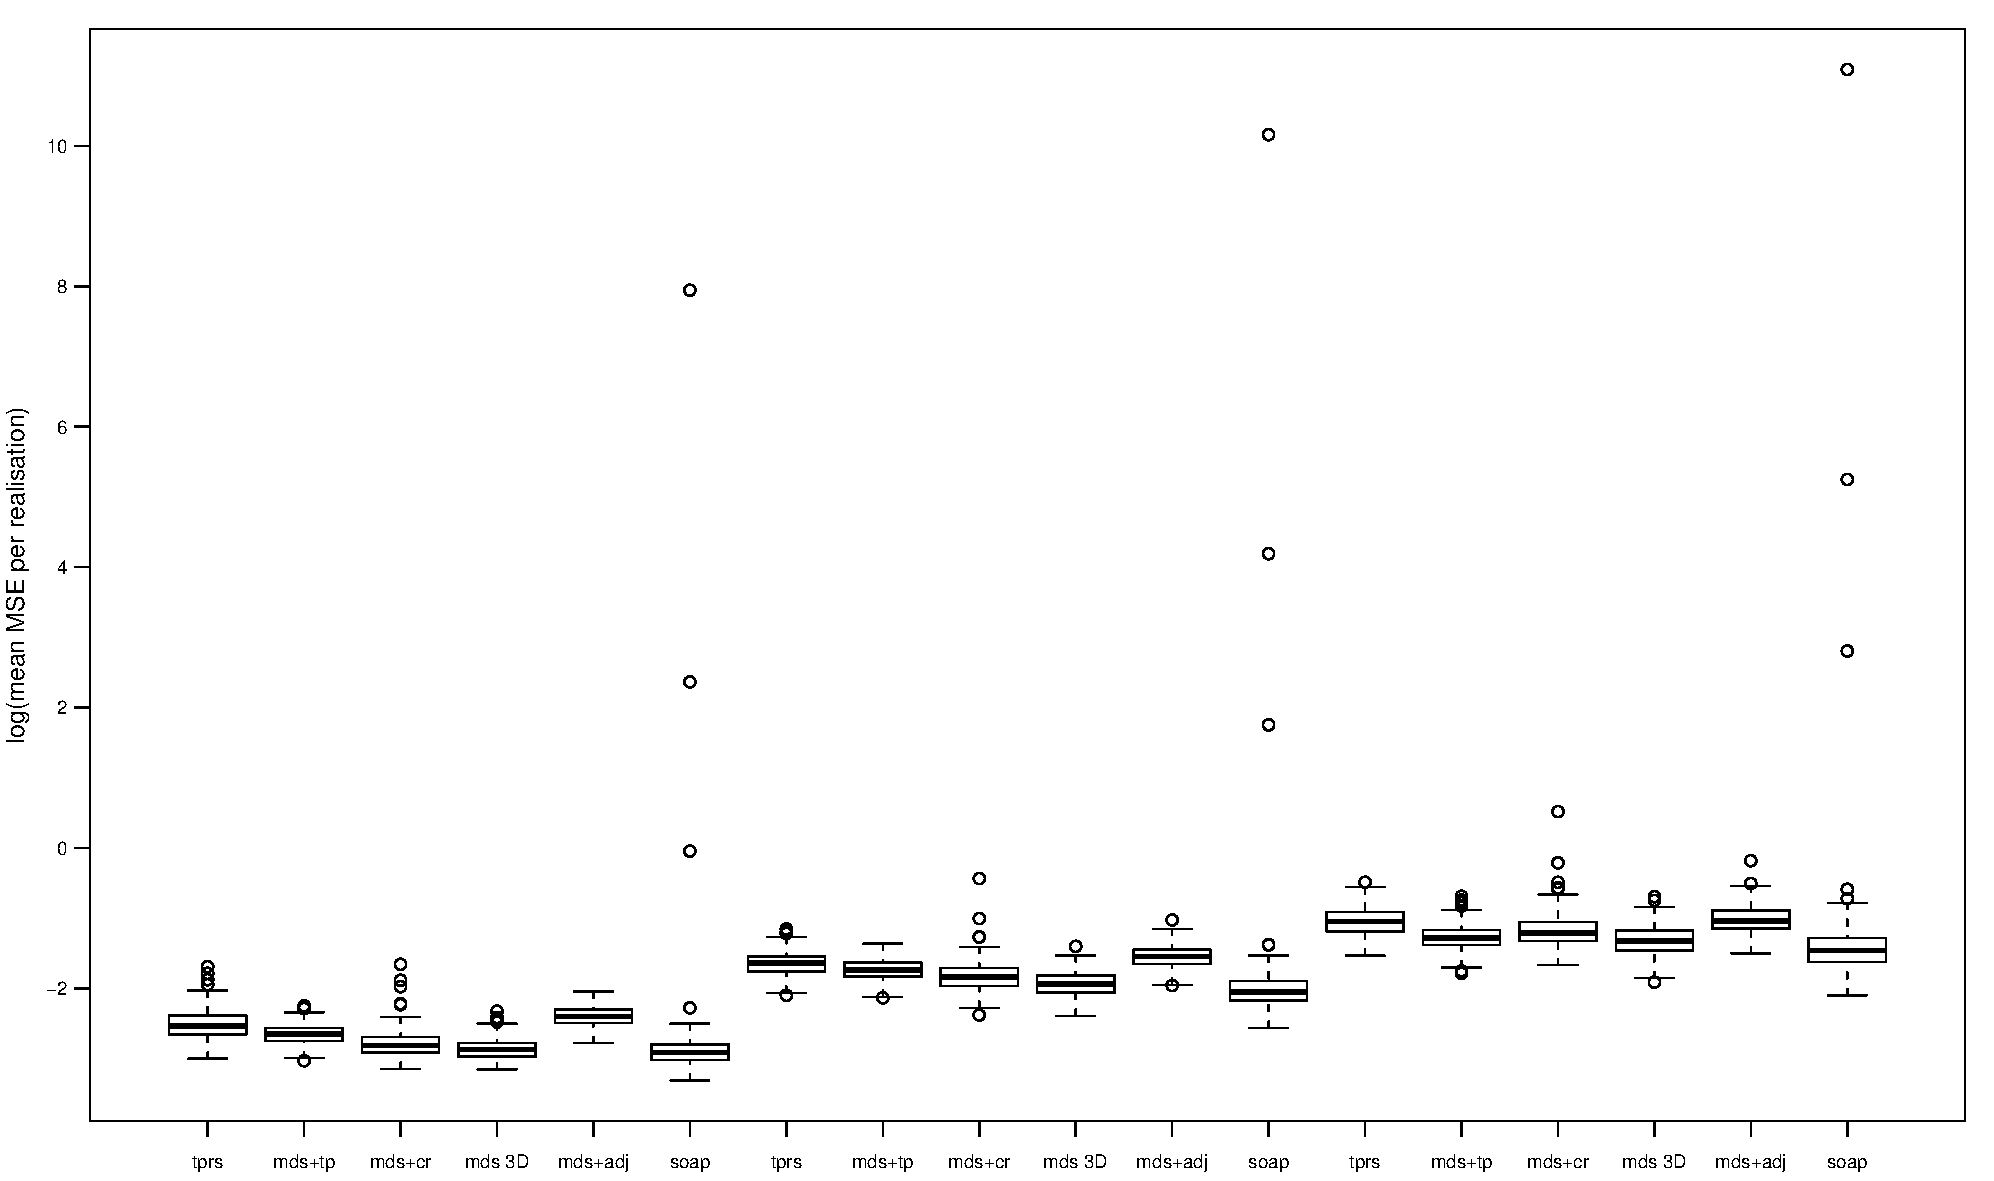
\includegraphics[width=\textwidth]{mds/figs/big-mds-wt2-boxplot.pdf} \\
\caption{Logarithm of per realisation average mean squared error for the double peninsulae domain. Models are in groups of five for each error level (0.35,0.9,1.55). In all cases, a Wilcoxon signed rank test showed that MSEs for all models were significantly different from the soap film smoother (at the 0.01 level).}
\label{big-wt2-mses}
% generate /phd-smoothing/mds/sim/boxplot-wt2.R
\end{figure}

% big wt2 sim MSEs
\begin{figure}
\centering
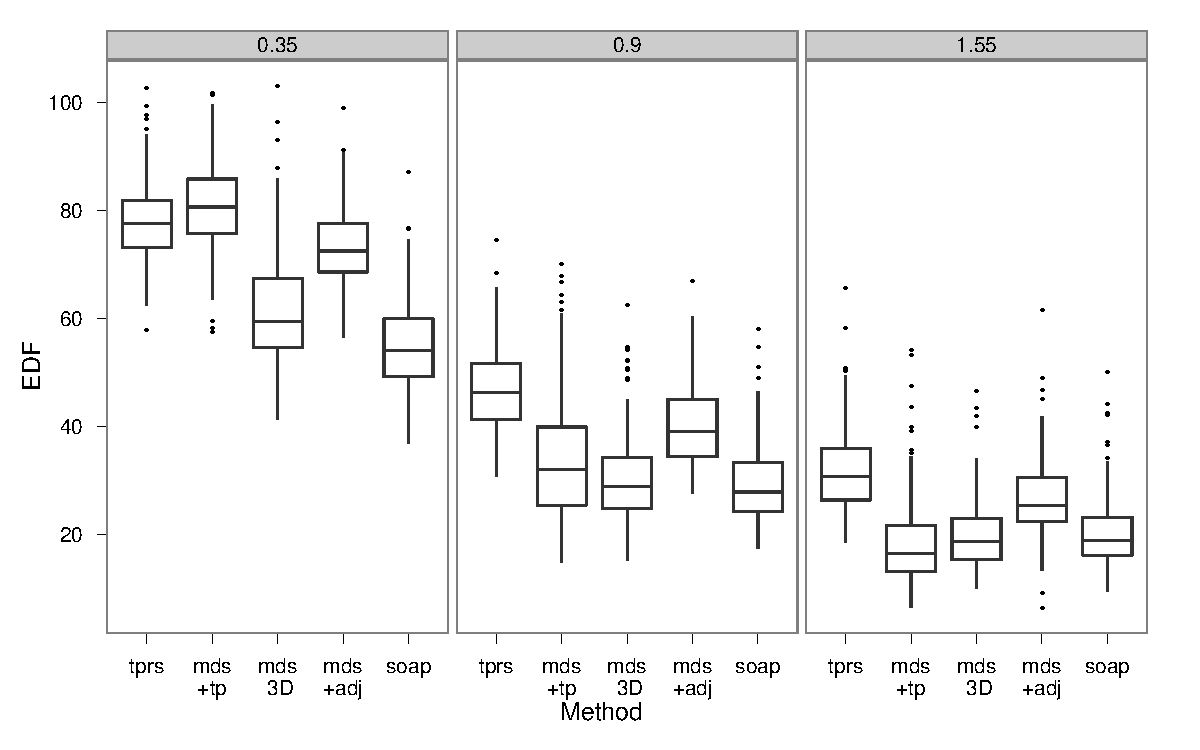
\includegraphics[width=\textwidth]{mds/figs/big-mds-wt2-boxplot-edf.pdf} \\
\caption{Per realisation EDFs for the double peninsulae domain. Models are in groups of five for each error level (0.35,0.9,1.55).}
\label{big-wt2-edfs}
% generate /phd-smoothing/mds/sim/boxplot-wt2-edf.R
\end{figure}



\subsubsection{Aral sea}
\label{aral-sec}

The Aral sea is located between Kazakhstan and Uzbekistan. It has been steadily shrinking since the Soviet government diverted the sea's two tributaries in order to irrigate the surrounding desert during the 1960s. The NASA SeaWifs satellite collected data on chlorophyll levels in the Aral sea (\cite{soap}) over a series of 8 day observation periods from 1998 to 2002. The 496 data are averages of the $38^\text{th}$ observation period. Smooths were fitted to the spatial coordinates (Northings and Easting projected from latitude and longitude) with the logarithm of chlorophyll concentration (with Gamma errors) as the response.

A \tprs, \mdsap\ and soap film were all fitted to the data. In summary the setup for each model was:

\begin{enumerate}
\item \emph{tprs}: thin plate spline with basis size 70.
\item \emph{soap}: the soap film smoother using a 12 by 12 grid of knots (74 were inside) and a boundary smooth with basis size 49.
\item \emph{mds}: \mdsap\ using thin plate regression splines with basis size 70.
\end{enumerate}

\begin{figure}
\centering
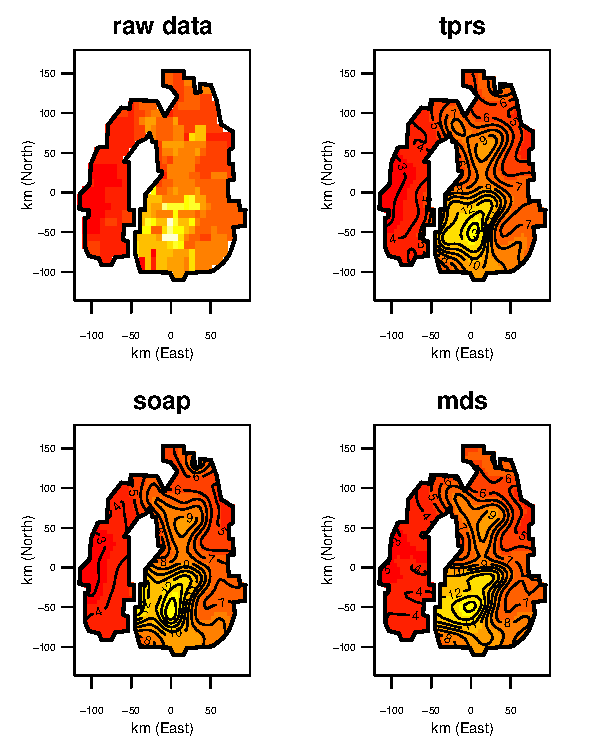
\includegraphics{mds/figs/aral-fit.pdf} \\
\caption{Raw data and predictions from the models fitted to the Aral sea chlorophyll data. Clockwise from top left: raw data, \tprs, soap film smoother, and \mdsap.}
\label{aral-fit}
% generated by phd-smoothing/mds/wt2-intexp.R and intexp/smooth2.c.R with comments removed
\end{figure}

The models were then used to predict over a grid of 496 points to create the heat maps shown in \fig{aral-fit}. The fits are broadly similar, with the \tprs\ showing some signs of leakage around (-50,-50). Both \mdsap\ and the soap film smoother combat this problem. The contour lines for all of the models look roughly the same in the main part of the sea, but in the smaller lobe, \mdsap\ is rather different from both the soap film and \tprs. 

Although the leakage is avoided, there appear to be some strange artefacts in the smooth. Ovals of higher chlorophyll appear in the smaller lobe when the \mdsap\ is fit to the data, along with contours close to the far left of the smaller lobe. Looking at a point plot in MDS space (\fig{aral-pp}) reveals why this might be happening. As can be seen from the figure, the smaller lobe has been severely squashed which will clearly have an adverse effect on the smoother.

\begin{figure}
\centering
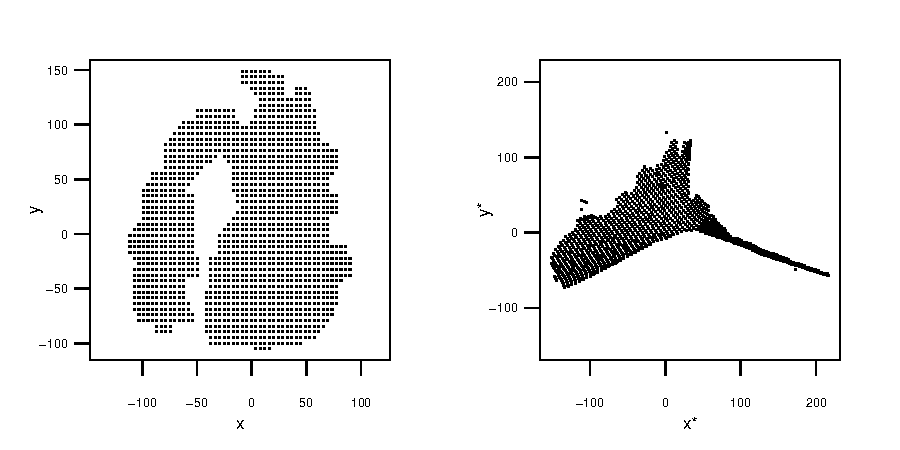
\includegraphics[width=\textwidth]{mds/figs/aral-pp.pdf} \\
\caption{The prediction points for the Aral sea data set (left), with their projection into MDS space (right).}
\label{aral-pp}
% generated by phd-smoothing/mds/aral/pointplot.R
\end{figure}

The \mdsap\ with adjusted penalty was also used to fit the model, using the same basis as above. The predicted surface given by the model is shown in \fig{aral-adj-fit}. Again, the same artefacts are clearly visible in the smaller lobe of the region.

\begin{figure}[t]
\centering
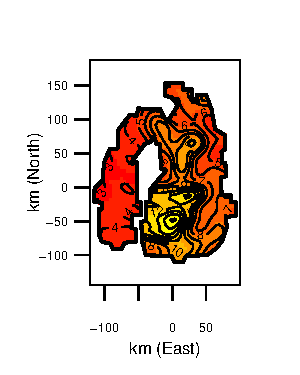
\includegraphics[width=3in]{mds/figs/aral-adjfit.pdf} \\
\caption{Predictions for the Aral sea using \mdsap\ with adjusted penalty.}
\label{aral-adj-fit}
% generated by ???
\end{figure}

Using a 3-D \tprs\ the artefacts are less prominent and the surface looks much more like the one given by the soap film smoother. Again, the three-dimensional projection shows much promise especially given the minimal extra cost to running the additional model (if the within-area distances are already calculated, only the MDS projection needs to be calculated, and the \tprs\ fitted).

\begin{figure}
\centering
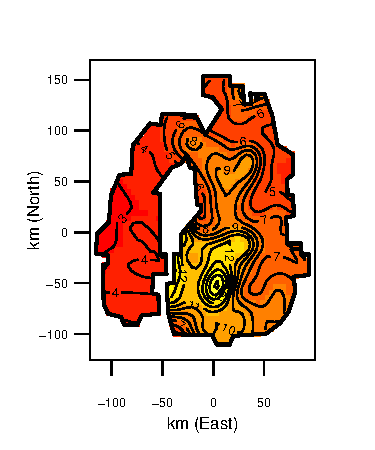
\includegraphics[width=3in]{mds/figs/aral-3d.pdf} \\
\caption{Predictions for the Aral sea using a 3-dimensional projection into MDS space with \mdsap.}
\label{aral-fit-3d}
% generated by ???
\end{figure}

\section{Problems with the methodology so far}
\label{mds-problems}

At this point two outstanding issues must be addressed. The first is that, following the experiments above, there are issues with artefacts in the smooths produced by \mdsap\ when a low dimensional projection is used. The effect of these artefacts is decreased when the projection is taken into higher dimensions, however, the artefacts are still problematic in some way and high dimensional smoothing can be rather tricky. 

What follows is an explanation of why the artefacts occur, and how high dimensional smoothing can help. This section explores these two problems, explains what is going wrong and sets out what is needed for a solution.

\subsection{Why adjusting the penalty is not the solution}
\label{pensuck}

The simulations show that when using \mdsap\ there is no big advantage of using the adjusted penalty scheme over the non-adjusted one. Before running the simulations, several different functions of the MDS point density ($\mathcal{L}^*$) were compared. All resulted in worse smooths (in MSE terms) than the function that was finally settled on.

Investigating the good performance of the 3-D projection model goes some way to explaining why the penalty adjustment doesn't offer much improvement.

Looking at the plots of the prediction points in MDS space for the peninsulae domain (\fig{wt2-2d-proj} and \fig{wt2-3d-proj}) it is easy to see that in two dimensions, the first peninsula has been squashed to a line. 

By truncating $\tilde{\mathbf{X}}^*$ in the MDS procedure (\secref{MDStechdet}) the information in $\mathbf{D}$ relating to the width of the peninsula has been lost. Projecting into higher dimensions reduces the truncation (smaller eigenvalues of $\mathbf{D}$ and their corresponding eigenvectors are use to construct $\tilde{\mathbf{X}}^*$) and as such more information about the relative positions of the points is introduced (this can be seen for the peninsula domain in \fig{wt2-3d-proj}). The adjusted penalty attempts to account for this squashing by allowing a more flexible model to be fit in that area. However, what is not taken into account is that some of the points in the peninsula are projected on top of (or on the wrong side of) one another. In other words, the 2-dimensional MDS projection makes the points lose their ordering. 

As a simple, unidimensional example, take three points, $a, b, \text{ and } c$ in the top line of \fig{linedia}. The projection could squash them in the way shown on the second line, in this case the penalty adjustments as described in \citeb{wood2000} could be used to correct the model. However, with MDS the situation shown in the bottom line of \fig{linedia} (changing the order of $a, b, \text{and}\ c$) can occur. This phenomena is also mentioned in \citeb[pp. 572-573]{elements}.

In the MDS projection we can see this happening for the peninsulae domain in figure \ref{wt2-3d-proj}. The projection takes a side-on view of the peninsula, making the points lose their ordering. In this case, the penalty adjustment can't save the model. If the ordering of the points is not guaranteed, then the smoother's job is potentially impossible, especially when one thinks of a 2-D extension of \fig{linedia}.

\begin{figure}
\centering
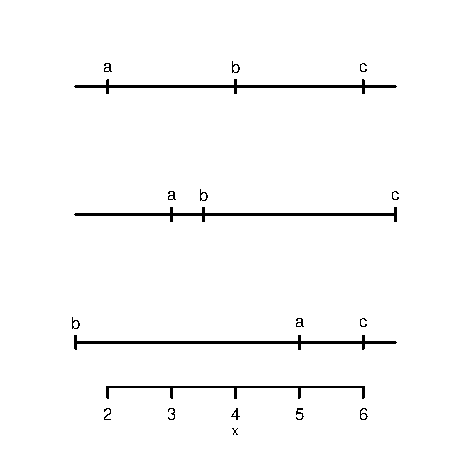
\includegraphics[width=3in]{mds/figs/linedia.pdf} \\
\caption{An illustration of how spatial mappings can squash points (middle line) and reorder them (bottom line) from their original configuration (top line).}
\label{linedia}
% generated by thesis/mds/figs/linedia.R
\end{figure}

\subsection{Why moving to higher dimensions is tricky}
\label{nohigherdim}

In the two cases above, moving into three dimensions allowed \mdsap\ to more accurately reproduce the true function. Counteracting the phenomenon above (where the ordering of the points is lost), the extra dimension allows us to see the ``width'' of parts of the domain that we take a side view of in the 2-D projection.

It seems then that there is some milage in taking a 3-dimensional projection to solve this problem without the need for penalty adjustments. However, unfortunately, this is not the case in general. \Fig{mds-comb} shows a long domain with three peninsulae at each end. The MDS projection of the domain in two dimensions gives the points in \fig{mds-comb-2d}. There are only four peninsulae in this figure, not the six which were in the original. Using the colours in \fig{mds-comb} and \fig{mds-comb-2d}, one can see the separation of the larger peninsulae and that the smaller peninsulae have been positioned end-to-end. Given that there could be interesting features in the response in these smaller peninsulae and that therefore leakage would be undesirable. This behaviour may well be worse than simply incurring leakage by using a standard smoother.

\begin{figure}
\centering
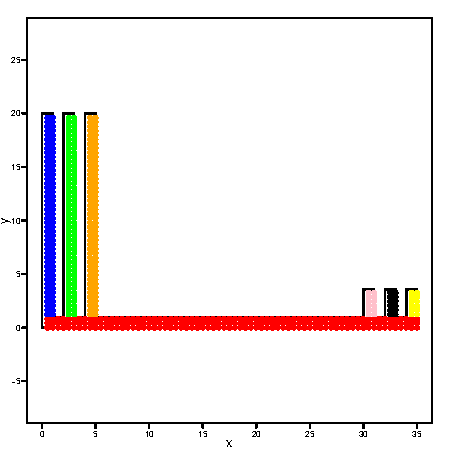
\includegraphics[width=3in]{mds/figs/comb.pdf} \\
\caption{The ``comb'' domain from \secref{nohigherdim}.}
\label{mds-comb}
% generated by thesis/mds/figs/comb.R
\end{figure}

\begin{figure}
\centering
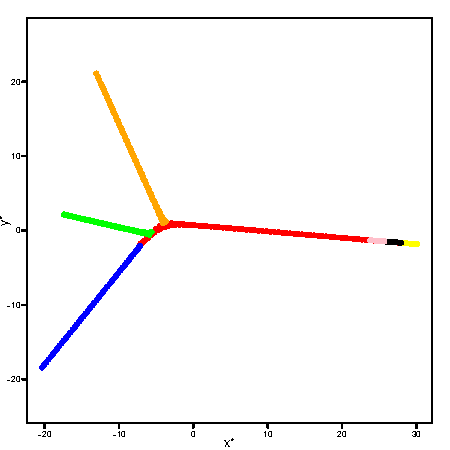
\includegraphics[width=3in]{mds/figs/comb-2d.pdf} \\
\caption{Two-dimensional MDS projection of the domain in \fig{mds-comb}, note that there are only four ``legs'' here not the six that should be there, as in \fig{mds-comb}.}
\label{mds-comb-2d}
% generated by thesis/mds/figs/comb.R
\end{figure}

Adding an extra dimension could help. Taking a 3-dimensional projection, \fig{mds-comb-3d} is produced; however there is still no separation of the smaller peninsulae. Moving into four dimensions (\fig{mds-comb-4d}) we begin to see separation in the smaller peninsulae. However, even in four dimensions the separation is not particularly large and leakage could still occur.

\begin{figure}
\centering
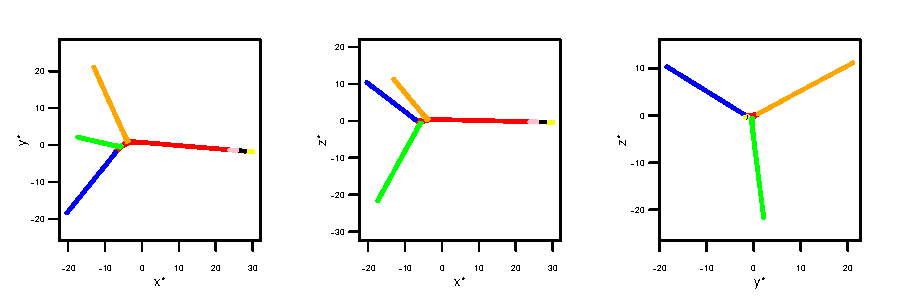
\includegraphics[width=\textwidth]{mds/figs/comb-3d.pdf} \\
\caption{The MDS projection of the domain in \fig{mds-comb} into three dimensions. Note that there is still no separation in for the smaller peninsulae.}
\label{mds-comb-3d}
% generated by thesis/mds/figs/comb.R
\end{figure}

\begin{figure}
\centering
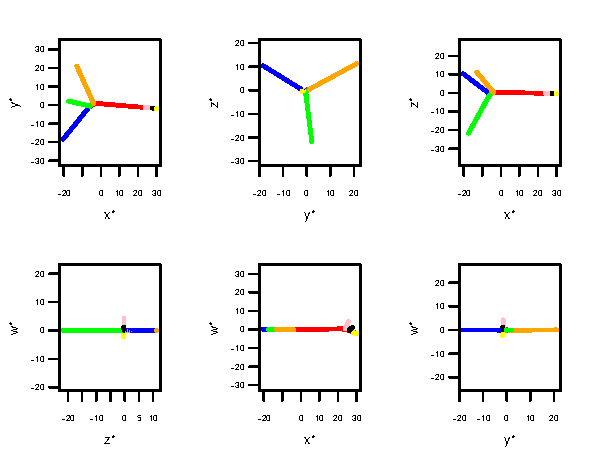
\includegraphics[width=6in]{mds/figs/comb-4d.pdf} \\
\caption{The MDS projection of the domain in \fig{mds-comb} in four dimensions.}
\label{mds-comb-4d}
% generated by thesis/mds/figs/comb.R
\end{figure}

Although these plots are illustrative, a quantitative measure of how well the within-area distances are being approximated by the MDS projection is desirable. Given the eigen-decomposition attempts to minimise the spectral norm, this is the logical metric to use. The spectral norm may be calculated as the the square root of the largest eigenvalue of $\mathbf{D}-\mathbf{D}_\text{E}$ where $\mathbf{D}$ is the matrix of within-area distances (as above) and $\mathbf{D}_\text{E}$ is the matrix of Euclidean distances in MDS space.

% Results here are in mds/counter/run-DRcomp.R
Looking at this measure for the domain considered in this section (the ``comb''), peninsulae domain (from \secref{mds-wt2-sim}) and the Aral sea as dimension of projection is increased yields some interesting results. These are summarised in figure \ref{increasek}. The plot indicates that there is some optimum number of dimensions ($k$) to project into, such that adding a further dimension gives only a negligible decrease in the spectral norm. 

The ``optimal'' $k$ (in a spectral norm sense) is not common to all of the domains. For the peninsulae domain there is a large decrease (roughly halving each time) up to four dimensions, but the Aral sea appears to settle down after three. However, it's clear that the spectral norm is not the best guide for this given that for the ``comb'' domain, four dimensions appears to be optimal but \fig{mds-comb-3d} shows that this doesn't offer much separation in the peninsulae. The spectral norm doesn't offer a direct solution to the issue of dimension selection but it does at least offer the insight that there is some dimensional beyond which an increase in dimension only offers marginal returns. Considering dimension selection separately from smoothing is sure to cause difficulties, since a point set that approximates the distances in $\mathbf{D}$ well does not give an guarantees about the quality of the resulting smooth. It seems that a dimensional selection method that also takes into account the response will be useful in this case.

%\begin{table}[htb]
%\centering
%\begin{tabular}{c c c c c}
%$k$ & Comb  & Peninsulae & Aral\\ 
%\hline
%1  &  3610.210  &  109.134  &  1519.736 \\ 
%2  &  1280.189  &  54.603  &  347.221 \\ 
%3  &  459.946  &  22.068  &  128.202 \\ 
%4  &  457.163  &  12.166  &  119.549 \\ 
%5  &  456.07  &  10.237  &  117.643 \\ 
%6  &  452.436  &  9.958  &  116.668 \\ 
%7  &  450.934  &  9.873  &  116.167 \\ 
%8  &  450.559  &  9.853  &  115.596 \\ 
%9  &  449.883  &  9.79  &  115.309 \\ 
%10  &  449.463 &  9.747  &  115.188 \\ 
%\end{tabular}
%\caption{Mean squared difference between the matrix of within-area distances and Euclidean distance in a $k$-dimensional MDS projection of the points for each of the domains detailed in \secref{nohigherdim}.}
%\label{increasek}
%\end{table}

\begin{figure}
\centering
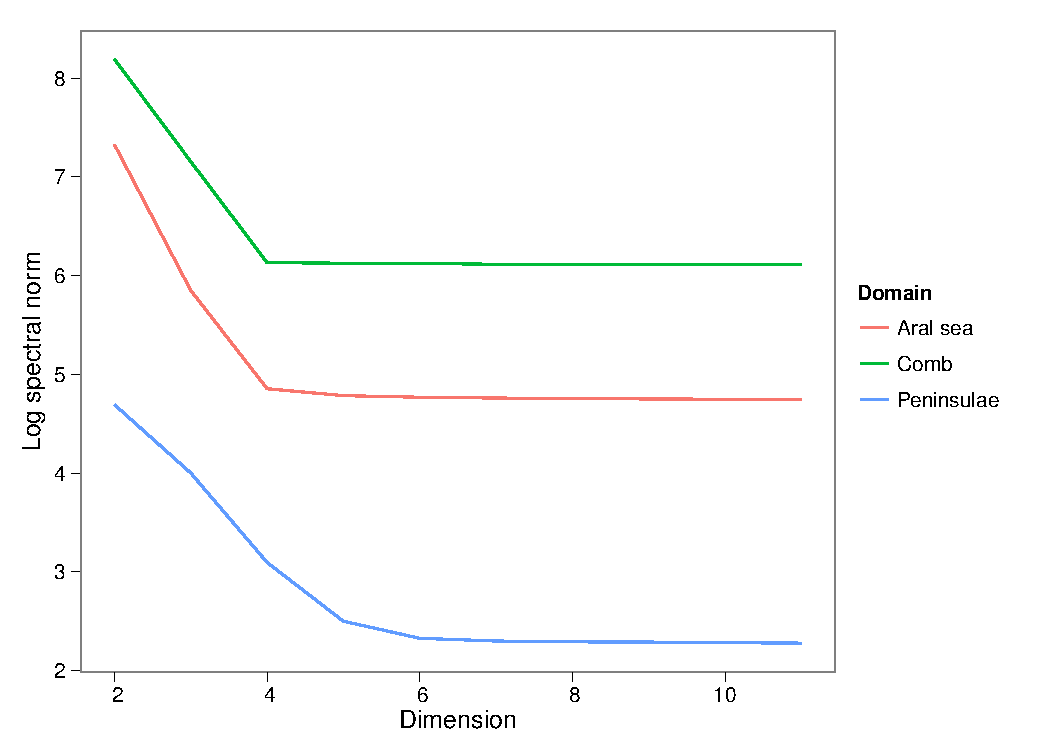
\includegraphics[width=\textwidth]{mds/figs/eigenplot.pdf} \\
\caption{Logarithm of the spectral norm of $\mathbf{D}-\mathbf{D}_E$ versus dimension for each of the domains detailed in \secref{nohigherdim}.}
\label{increasek}
% generated by thesis/mds/figs/eigenplot.R
\end{figure}



Moving into continually higher dimensions is appealing, but practically it is rather more taxing. As the dimension of the problem is increased, the order of the derivative in the spline penalty increases too (see \secref{GAMpenalties} and \secref{gds-tprstoduchon}). As this happens, the dimension of the nullspace of the penalty increases, meaning that both the number and complexity of the unpenalised functions in the model increases. An increasingly large space of unpenalized functions is certainly unappealing, but the next chapter will investigate how to work around such issues.

\section{Conclusion}
\label{mds-conc}

This chapter has investigated the utility of using a combination of multidimensional scaling and penalised regression splines to combat the phenomenon of leakage in spatial smoothing. This was with a view to \mdsap\ being a less complex, faster, alternative to soap film smoothing, with an equally interesting motivating physical model.

Considering these goals, first, the model certainly seems less complex. Provided that one knows about spline smoothing (which one would have to know to use soap too) and about multidimensional scaling (which is commonly taught outside of statistics, in biology, ecology or computer science) the method is relatively easy to get to grips with. No understanding of differential equations is required, nor is there any need to create knots (unlike soap film smoothing). The physical model is still quite close to that which was outlined in \secref{intro-leakageapproaches} part 4: the idea of morphing the domain into a shape which does not suffer from leakage.

In comparison to using the \sch\ transform, \mdsap\ has the disadvantage of not being a functional mapping. Having a fixed functional form makes the \sch\ transform extremely fast since only a single function evaluation is needed to map a single point. In comparison, having to find the within-area distances is rather involved. However, the speed-ups presented in \secref{mds-faster} greatly enhance the utility of the method from a practical viewpoint. \mdsap\ and soap film smoothing differ in how their computational time is divided. The main computational burden of the soap film smoother is in solving the PDEs needed to form the basis and from that calculating the penalty matrix (see table \ref{wt2itime} and part 3 of \secref{intro-leakageapproaches}), prediction is merely a case of evaluation. \mdsap\ on the other hand, spends the bulk of its computational time on finding the within-area distances for both fitting and prediction (comparing the ``thin plate'' and ``MDS+RS(\textit{pp})'' columns of table \ref{wt2itime}). The advantage of this is that since the distance calculation is effectively a black box from the perspective of the smoothing, if a faster routine for distance calculation were to be used there would be no difference in the results (provided that the routine calculated the distances exactly and did not rely on a discritization of the domain) but the computational time to calculate the final smooth would be significantly reduced. This approach also opens up the possibility of other distance metrics being used to form the distance matrix (as will be seen in \secref{gds-gds-examples}).

Figures \ref{wt2-3d-proj} and \ref{aral-pp} show that MDS does achieve the kind of domain morphing that was sought in section \ref{sc-conclusions}. Unlike the \sch\ transform, the projection does not force the points to move into a fixed transformation domain an as such avoids some of the issues with point density. 

Using MDS to re-arrange the points does not entirely work around the problem of squashing. Although there is no numerical crowding (see \secref{sch-crowding}), points may still have an uneven spatial distribution, which causes problems for isotropic smoothers like the thin plate spline. \Secref{mds-penadjust} sought to avoid the problems that occur when the space in which smoothing is to be performed by adjusting the penalty based on the density of the points. This did not work because of the confounding issue of point ordering (as discussed in \secref{pensuck}). The varying point density and ordering problems were due entirely to using a low dimensional projection in MDS space. Ensuring that point ordering is maintained and that the point density remains roughly even can be controlled by the projection dimension. This theme will be continued in the next chapter.

As we have seen over the last two chapters, although domain transformation methods are appealing from a mathematical and physical point of view, in practise they are tricky to apply and can produce artefacts in the resulting smooths. These artefacts can be avoided by moving into higher dimensions where the ordering of the points is not disrupted. The potential problem of using higher dimensional projections is that model parsimony is jeopardised by an increasingly complex nullspace. In the next chapter the use of high dimensional MDS projections will be investigated when an appropriate spline basis can be used to perform smoothing. If reliable high dimensional smoothing can be performed, then the only remaining issue is to resolve the issue of projection dimension selection, the next chapter will deal with this too.
